\documentclass[conference]{IEEEtran}
%\IEEEoverridecommandlockouts
\usepackage{amsmath}
\usepackage{amssymb}
\usepackage{graphicx}
% \usepackage[subtle]{savetrees}
% \usepackage{authblk}
\usepackage{float}
\usepackage{graphicx}
%\usepackage[colorinlistoftodos]{todonotes}
%\usepackage{todonotes}
%\usepackage{soul}
\usepackage{algorithm}
\usepackage[noend]{algpseudocode}
\usepackage{subcaption}
%\usepackage[hyphenbreaks]{breakurl}
\usepackage[hyphens]{url}
%\renewcommand{\baselinestretch}{0.87}

%\graphicspath{ {c:/Users/mjutras/TeXworks/images/} }
\graphicspath{ {images/} }

% \author[6]{Deon Burchett, PhD}
%author[5]{Brady Collea}
% \author[3]{Melanie Jutras}
% \author[2]{Les Servi, PhD}
% \author[1]{Randy Paffenroth, PhD}

% \affil[1,2,3,4]{The MITRE Corporation}
% \affil[5]{Worcester Polytechnic Institute}

\begin{document}

\title{Reducing Reporting Burden of Healthcare Data Using Robust Principal Component Analysis}

% My title isn't perfect but I think it is closer.  Let';s get it even better
%\title{Minimizing the Burden of Measuring Healthcare Data with Robust PCA}

% \author{\IEEEauthorblockN{ANONYMOUS}
% \IEEEauthorblockA{Anonymous\\
% Anonymous \\ 
% Anonymous \\
% Email: Anonymous}
% }

\author{\IEEEauthorblockN{1\textsuperscript{st} Les Servi}
\IEEEauthorblockA{
\textit{The MITRE Corporation}\\
Bedford, MA, USA \\
lservi@mitre.org}
\and
\IEEEauthorblockN{2\textsuperscript{nd} Randy Paffenroth}
\IEEEauthorblockA{\textit{Mathematical Sciences,} \\
\textit{Computer Science} \\
\textit{and Data Science} \\
\textit{Worcester Polytechnic Institute}\\
Worcester, MA, USA \\
rcpaffenroth@wpi.edu}
\and
\IEEEauthorblockN{3\textsuperscript{rd} Melanie Jutras}
\IEEEauthorblockA{
\textit{The MITRE Corporation}\\
Bedford, MA, USA \\
mjutras@mitre.org}
\and
\IEEEauthorblockN{4\textsuperscript{th} Deon Burchett}
\IEEEauthorblockA{
\textit{The MITRE Corporation}\\
Bedford, MA, USA \\
deonb@mitre.org}
}

% \author{\IEEEauthorblockN{Les Servi}
% \IEEEauthorblockA{The MITRE Corporation\\
%  202 Burlington Road \\ 
% Bedford, MA 01730-1420 \\
%  lservi@mitre.org}
% \and
% \IEEEauthorblockN{Randy Paffenroth}
% \IEEEauthorblockA{
% %Mathematical Sciences, \\
% %Computer Science, \\
% %and Data Science\\
% Worcester Polytechnic Institute\\
% 100 Institute Rd, \\
% Worcester, MA 01609 \\
%  rcpaffenroth@wpi.edu}
% %   \and
% % \IEEEauthorblockN{Melanie Jutras}
% % \IEEEauthorblockA{The MITRE Corporation\\
% % 202 Burlington Road \\ 
% %   Bedford, MA 01730-1420
% %  Email mjutras@mitre.org} 
%   \and
%  \IEEEauthorblockN{Melanie Jutras} 
% \IEEEauthorblockA{The MITRE Corporation\\
% 202 Burlington Road \\ 
%  Bedford, MA 01730-1420 \\
%  mjutras@mitre.org} 
%     \and
%  \IEEEauthorblockN{Deon Burchett}
% \IEEEauthorblockA{The MITRE Corporation\\
% 7525 Colshire Drive \\ 
%  McLean, VA 22102-7539 \\
%  deonb@mitre.org} 
% }

\maketitle

% FIXME: Remove before submissions!  This is just to keep track of the length as we write.
\thispagestyle{plain}
\pagestyle{plain}
%\todo[inline]{RCP: Remove page numbering before submission}

\begin{abstract}
%\todo [ color = red]{LS: MITRE ask:The entire background section has no citations. Usually there is a citation that corroborates your claims that there is an actual problem. DONE but citation needs to be fixed }
%\todo [ color = red]{LS notes:  looks useful as does 
%https://blog.ncqa.org/meahttps://www.healthit.gov/sites/default/files/page/2018-11/Draft%20Strategy%20on%20Reducing%20Regulatory%20and%20Administrative%20Burden%20Relating.pdfsurement-burden-heres-what-we-told-onc/} 

%\todo [color = red]{LS: MITRE ask: Are you saying that you can’t reduce the reporting burden %until after the data is already reported, when you can do the analysis of correlations? %Theoretically this will reduce the burden %the following DONE}

The US government imposes reporting requirements on healthcare providers as health metrics are important for assessing and improving the US healthcare system.  However, proposed health metrics requirements can be unnecessarily burdensome if the preliminary analysis does not consider possible redundancies between the various metrics.  Accordingly, if some subset of the proposed metrics could be demonstrated to contain nearly all the information of  the full set of metrics,
% (e.g.,  having the subset permits one  to accurately predict the values of the metrics outside the subset)
then the reporting burden could be substantially  lightened with minimum impact.  However, such an analysis is complicated by anomalies in the collected metrics.  Accordingly, we propose a machine learning approach which simultaneously identifies redundancies in collected healthcare metrics and identifies anomalies in those collected metrics.
\end{abstract}

\begin{IEEEkeywords}
robust principal component analysis, anomaly
detection, health analytics, dimension reduction
\end{IEEEkeywords} 

\section{Introduction}

\subsection{Background}
%\todo[color=orange]{DONE: 8 Jul 2020:  This section was rewritten by LS.  I think it is in good shape but it would be nice for RP to quickly review it. }

Government agencies  mandate  metric reporting requirements to help them execute their missions.  In particular,  metrics are required for the evaluation of healthcare systems and initiatives in order to improve healthcare safety, quality and value. However, collecting and managing healthcare quality measures is expensive,  time consuming and prone to inaccuracies \cite{rao2017impact, cutler2012reducing}.  These inaccuracies take two forms.  Some inaccuracies are caused by the reality that attempts at precise metrics are not always met whereas others are wildly anomalous due to transcription errors, a misunderstanding of the precise requested metric or other business process errors.

The need for lessening the mandated reported metrics has long been recognized yet is still a concern.  For example, in 2016, Congress passed the  21st Century Cures Act\footnote{H.R. 34, Public Law 114-255, Section 4001 - Dec. 13, 2016} which identified the importance of easing regulatory burden with the use of electronic health records, EHRs, and required  the Department of Health and Human Services to publicize a strategy, seek public comments and then published a finish set of recommendations to reduce the burden. \cite{HHS2019str} The recommendations were strategic in nature. One recommendation was to "reduce the effort and time required to meet regulatory reporting requirements for clinicians, hospitals, and health care organizations."  This paper presents a machine learning approach to assist with this recommendation. 


An existing set of health metrics may be unnecessarily large and onerous because the initial analysis to design the metrics did not properly account for redundancy of information between metrics \cite{lesidea1, vostok2013assessment}.
%\todo[color=yellow,]{8 Jul  find details }Ref AcademyHealthAbstract].LS thinks we should DROP this} 
Identifying such redundancies using standard methods revolving around computing correlations between the proposed metrics is hampered because the inevitable inaccuracies in the data will give a false sense of the correlations and underlying dimensionality of the metrics.   Instead, more advanced methods are required to effectively correct for  inaccuracies in the data, identify and remove anomalous metric measurements, and only then examine the resulting correlations and dimensionality structure.

A promising data driven analytical approach to reduce metric reporting requirements burden without compromising the information which can be gleaned from the data is reported in this paper. This approach is applied to real data of  health metrics obtained from public use files collected over a period of one year.  However to validate the approach it was also applied to synthetic data where ground truth is known and both small errors and anomalous errors were intentionally inserted.


\subsection{Contribution}
%\todo [ color = red,inline] { 28Aug: LS reread this and made numerous small change.  Please do same.  I want a less technical person to basically understand the capability developed from this section}
\subsubsection{Overview}
This paper has the methodological contribution of extending previous Robust Principal Component Analysis (RPCA) research \cite{paffenroth2018robust,Paffenroth2012} (and references therein) and using it in a new manner to address the practical reporting burden challenge.  Specifically,  the new approach  algorithmically ingests training data and then removes data anomalies while more accurately identifying its underlying low-rank structure. This, in turn, provides as pathway to reducing the reporting requirements with minimal adverse impact. A straightforward application of Robust Principal Component Analysis (RPCA), and even more so with classical PCA, would lead to large rank structure and hence a  larger reporting requirement without compensating added information.  While in principle other machine learning methods revolving around neural networks or deep learning might be used to try to address the reporting requirement challenges, extensions of RPCA extended and combined in new ways is structurally designed to be focused on low rank identification and anomaly removal and hence is the approach adopted.   While the approach  is presented in the context of healthcare metrics it is more broadly applicable.  %  The details for the algorithms that underlie this work can be found in \cite{paffenroth2018robust,Paffenroth2012} (and references %therein), and here we focus on the application of such algorithms to the particular nuances of healthcare metrics. 

%\todo[color = yellow,inline] { Discuss Randy's new table of MSE and estimated rank (and then ask Randy to look at it) LS is confused: it from Table 1 it looks like PCA and RPCA is better than SPCA and RPCA }
\subsubsection {Illustrative Specific Contribution}
In particular, empirical examples on synthetic data show that combining Sparse Principal Component Analysis (SPCA) with RPCA preprocessing was the only method tested herein that found all possible anomalies 
%and led to an MSE in reconstructing as low as possible. 
and correctly determined the minimum metric reporting burden. For example, we considered the case of $100$ testing facilities with $20$ metrics each (but for which only $6$ would have sufficed). It succeeded in correctly determining the minimum metric reporting burden even when we  complicated our task by adding $5$ anomalies to the  data sets.  This was accomplished by first using RPCA  to identify in the training set the reduced dimensional space of the parameters without being distracted by the anomalies present.  With this preprocessing SPCA was successfully applied to a test data set analysis by SPCA had an accurate reconstruction of the metrics recommended to not be required.  
%\todo [color = orange,inline] {RP: Should we add to the table the number of anomalies found as well as the number of false detections for each methods?  RP:  That is, effectively, contained in the F1-score table.}
Specifically, as shown Table \ref{tab:table2} the SPCA with RPCA approach detected all anomalies  and, as shown in Table \ref{tab:table1},  discovered that the burden of measuring could have been reduced from $20$ metrics to only $6$ as the MSE values while incurring insignificant loss of the ability to reconstruct the original true metric values in absence of anomalies and with a small loss of ability to reconstruct the original data when anomalies were present.  It is important to note that, as shown in Table \ref{tab:table2}, the combination of PCA and RPCA provides a slightly lower error than our proposed combination of SPCA and RPCA.  However, the PCA and RPCA combination \emph{require the measurement of all metrics and provides no reduction of the reporting burden.}  Finally, in  Figure \ref{fig:real_data}, we demonstrate the effectiveness of our approach on real-world healthcare metrics.   As this is real-world data we do not have access to the ground-truth for anomaly detection.  However, for an appropriate choice of our regularization parameter $\lambda$ we \emph{successfully detect all artificial anomalies we inject into the real-world data as well as a number of measured data points that are anomalous based upon our model.}
%, with no false alarms, all anomalies which permitted the algorithm to discover that the burden of measuring could have been reduced from $20$ metrics to only $6$ without \emph{any} appreciable loss of information.  
%\todo [color = green,inline]{LS: MITRE ask: Clearly this is for a very specialized audience, because those %figures don’t
%make a whole lot of sense to me. As such, the point you are trying to make
%is not well served.28 Aug: This was based on a prevoius draft.  LS doesn't think this is an issue any longer}

% \todo [ inline, color = yellow] { Need to, in words, explain what PCA alone means and SPCA alone means }

%\todo [ inline, color = yellow] { Need to also summarize Fig 8, ie state we are using real data and this is what we were able to do with it.   }
Figures \ref{fig:error_PCA_prediction_without_RPCA} and
\ref{fig:error_SPCA_prediction_without_RPCA_first_selected} demonstrate that competing methods either mis-detect the anomalies, incorrectly predict the non-anomalous entries, or get the required number of required metrics incorrect.
As shown in Figure \ref{fig:error_SPCA_prediction_with_RPCA_first_selected} our method can be seen to be the only method that accomplishes all three tasks (anomaly detection, correctly computing the number of required metrics, and reconstructing the complete data set).  We examine using both PCA and SPCA for dimensionality reduction and, for both methods, we examine their effectiveness both  with and without RPCA preprocessing (for a total of $4$ different approaches).
In particular, empirical examples show that the combination of SPCA and RPCA was the only method to reconstruct the non-measured metrics to an RMSE of approximately $0.2$\% while at the same time having an F1-score for the anomaly detection of $0.99$, even when the anomalies are of a size similar to the ambient non-anomalous measurements.  
\subsubsection {Summary}
%\todo[inline, color = yellow] {What do we do with this reference to newPaper?  RCP DONE!  I used my original RPCA paper and our arxiv.org paper.   If, however, you mean the upcoming that has not even been started yet, I don't think that we can cite it. }
%\todo[inline, color = yellow]{ Might be nicer to make punchier and more quantitative, e.g. "In particular, empirical examples show it found XX more anomalies, and led to XX better MSE in reconstructing original dataset. RCP needs to write some code and redo some runs to get MSE numbers}
% \todo[inline]{RCP:  Add something about what made the synthetic problem hard, eg, N anomolous (M percent) which are on average size Y as well as noise of size Z thrown in.}
%\todo[color=red,inline]{RCP and LS:  Need to nail down this request "Also, need a sentence about real data: Had a %method to verify that it was catching anomalies and also showed that it appeared that we can reduce the metric %burden by X with minimal impact."}


In this paper we make several contributions.

\begin{itemize}
    \item We demonstrate how RPCA can be used to find anomalies in both synthetic and real data sets arising from healthcare metrics.   
    %which permits the SPCA to be very effective,
    \item We show how, once anomalies are identified, one may select a smaller subset of metrics from which the remaining metrics may be reconstructed.   Such an approach can be used to substantially reduce the reporting burden on healthcare providers while maintaining the richness of their provided information for downstream analysis.
    \item We apply these algorithms to both synthetic and real-world healthcare data sets to robustly select a subset of metrics that may be less expensively measured and detect anomalies in both training and testing data.
\end{itemize}
\bigskip
This paper is organized as follows:  Section \ref{anal} provides a technical background of approaches related to those used in this paper: (i) Traditional Principal Component Analysis (PCA), (ii) Sparse Principal Component Analysis (SPCA), and (iii) Robust Principal Component Analysis (RPCA). Next, the nature of the data will be reviewed: first the synthetic data used to explore the properties of the approach of this paper and then real data from the Centers for Medicare and Medicaid Servides (CMS). Next, the paper's new approach will be presented along with alternative approaches which will be numerical compared with. Finally, numerical comparisons using synthetic and real data will be presented and then the conclusions of the paper will summarize the findings.

\section{Analysis} \label{anal}
%\todo[color=red,inline]{LS: MITRE Ask: In contrast to what}
Data analysis was performed on both synthetic and real world data sets which will be described in the sections below. Analysis of synthetic data is particularly useful as we know the ground truth. Analysis of real world data sets is complicated by the fact that in many cases, we do not know ground truth.  This can make anomaly detection and dimension reduction difficult as we do not know what the outlier data points are and we also do not know the true rank of the data.


% \todo{should include bullet list}
% TBD TBD TBD TBD TBD TBD TBD TBD TBD TBD TBD TBD TBD TBD TBD TBD
% TBD TBD TBD TBD TBD TBD TBD TBD TBD TBD TBD TBD TBD TBD TBD TBD
% TBD TBD TBD TBD TBD TBD TBD TBD TBD TBD TBD TBD TBD TBD TBD TBD
% TBD TBD TBD TBD TBD TBD TBD TBD TBD TBD TBD TBD TBD TBD TBD TBD
% TBD TBD TBD TBD TBD TBD TBD TBD TBD TBD TBD TBD TBD TBD TBD TBD

% \begin{itemize}
% \item TBD TBD TBD TBD TBD TBD TBD TBD TBD TBD TBD TBD TBD TBD TBD TBD
% TBD TBD TBD TBD TBD TBD TBD TBD TBD TBD TBD TBD TBD TBD TBD TBD
% \item TBD TBD TBD TBD TBD TBD TBD TBD TBD TBD TBD TBD TBD TBD TBD TBD
% TBD TBD TBD TBD TBD TBD TBD TBD TBD TBD TBD TBD TBD TBD TBD TBD
% \item TBD TBD TBD TBD TBD TBD TBD TBD TBD TBD TBD TBD TBD TBD TBD TBD
% TBD TBD TBD TBD TBD TBD TBD TBD TBD TBD TBD TBD TBD TBD TBD TBD
% \end{itemize}

%\section{Background}
\subsection{Traditional PCA} \label{PCA}
%\todo[color=yellow,inline]{LS:  Update code to reflect that it is not true that the main concern about PCA is the %difficulty to interpret.  We don't like PCA because it reduces the dimension of the data but it doesn't reduce %the number of measurements we use. DONE}
%\todo[color=yellow,inline]{LS:  It would be great to work through this section since it was copied from our arxiv.org paper.  This is a different audience and we want to avoid self-plagarism. 28 AUg: LS made a number of changes which RP should review here}

Principal Components Analysis (PCA) addresses a challenge similar to reporting metric reduction but different.  Rather than recommend a specific  reduction of metrics, PCA recommends a smaller set of linear combination of metrics.  The latter is useful for understanding the rank or underlying dimension which provides perspective in selecting a reduction of metrics. Perhaps more importantly,  PCA is sometimes extremely sensitive to anomalous measurements.  One anomalous measurements in the data can completely change the results.  As such, any guidance from PCA can be distorted.
%\todo [color = yellow,inline]{28 AUg: LS wanted to change what is below but it is too well written to touch}
In particular, consider a collection of
points $\{x_0,...,x_m\}$ with $x_i \in \mathbb{R}^n$.  Herein we follow the notation and presentation in \cite{paffenroth2018robust} and refer the interested reader there for additional technical details.  However, for the present context
we note that each point above represents some object  of interest, such as the $n$ measured properties of some health-care provider. The set of points $\{x_0,...,x_m\}$ would therefore
represent the collection of health-care providers that we intend to analyze.
The goal of PCA is therefore to compute a linear projection of the points $\{x_0,...,x_m\}$ into a new
set of points $\{\hat{x}_0,...,\hat{x}_m\}$ that each lie on some $k$-dimensional subspace of the original
$n$-dimensional space.  Of course, one might rightly wonder if, for $k < m$ or even $k \ll m$, if there is any 
such subspace that is close to the original points.  However, as we will demonstrate here, such health-care provider is
actually quite redundant and does not, in fact, fill the whole $m$ dimensional space.

The idea is that the subspace is chosen such that each point $x_i$ has to be moved as little as possible
to make it lie on the $k$-dimensional subspace.  If one encodes the measurement $x_i$ into a matrix
$X \in \mathbb{R}^{m \times n}$ with each $x_i$ being a row of $X$, then one can find
the low-dimensional representation $X$ by solving an optimization problem such as 

\begin{align} \label{PCAopt}
  &\min_{L} \| L-X \|_F^2 \\ \nonumber
  \text{subject to}\quad & \rho(L) \le k
\end{align}

\noindent where $\| L-X \|_F^2$ is the sum of the squares of the entries of $L-X$ (often called the Frobenius norm), $L \in \mathbb{R}^{n \times m}$ and $\rho(L)$ is the \emph{rank} of $L$ (the dimension of the subspace spanned by the rows of $L$).

As is quite standard \cite{HastieTrevorTibshiraniRobertFriedman2009}, the optimization problem in (\ref{PCAopt}) is solved by way of the Singular Value Decomposition (SVD) \cite{Eckart1936}.  In particular, by the SVD we know that $X=U \Sigma V^T$ where, assuming that $n<m$, we have $U \in \mathbb{R}^{m \times n}$ and $U$ is unitary in that $U^T U = I$; $V \in \mathbb{R}^{n \times n}$ and $V$ is unitary in that $V^T V = I$; and $\Sigma \in \mathbb{R}^{n \times n}$ and $\Sigma$ is diagonal with positive diagonal entries $\sigma_i$ called the \emph{singular values} of $X$.

Further, assuming the singular values are ordered such that $\sigma_i \ge \sigma_{i+1}$
and, for a given matrix $X$, we denote by $X_{i:j,k:l}$ the principle sub-matrix of $X$ comprised of rows $i$ through $j$ and columns $k$ through $l$, it is also standard \cite{HastieTrevorTibshiraniRobertFriedman2009} to derive Principal Component Analysis as 

\begin{align*}
X 
& = 
\begin{bmatrix}
U_{1:k,1:k} & U_{1:k,k+1:m} \\
U_{k+1:n,1:k} & U_{k+1:n,k+1:m} \\
\end{bmatrix}
&
\begin{bmatrix}
\Sigma_{1:k,1:k} & 0 \\
0 & \Sigma_{k+1:n,k+1:n} \\
\end{bmatrix} \\
&
\begin{bmatrix}
V_{1:k,1:k} & V_{1:k,k+1:n} \\
V_{k+1:n,1:k} & V_{k+1:n,k+1:n} \\
\end{bmatrix} \\
\end{align*}

\noindent Now, by assumption, every entry of $\Sigma_{k+1:n,k+1:n}$ is smaller than the smallest
entry of $\Sigma_{1:k,1:k}$ we approximate $X$ by setting $\Sigma_{k+1:n,k+1:n}=0$
and get

\begin{align*}
X \approx 
\begin{bmatrix}
U_{1:k,1:k} & U_{1:k,k+1:m} \\
U_{k+1:n,1:k} & U_{k+1:n,k+1:m} \\
\end{bmatrix}
\begin{bmatrix}
\Sigma_{1:k,1:k} & 0 \\
0 & 0 \\
\end{bmatrix}\\
\begin{bmatrix}
V_{1:k,1:k} & V_{1:k,k+1:n} \\
V_{k+1:n,1:k} & V_{k+1:n,k+1:n} \\
\end{bmatrix} \\
= 
\begin{bmatrix}
U_{1:k,1:k} & 0 \\
U_{k+1:n,1:k} & 0 \\
\end{bmatrix}
\begin{bmatrix}
\Sigma_{1:k,1:k} & 0 \\
0 & 0 \\
\end{bmatrix}
\begin{bmatrix}
V_{1:k,1:k} & V_{1:k,k+1:n} \\
0 & 0 \\
\end{bmatrix} \\
= 
\begin{bmatrix}
U_{1:k,1:k} \\
U_{k+1:n,1:k} \\
\end{bmatrix}
\begin{bmatrix}
\Sigma_{1:k,1:k}
\end{bmatrix}
\begin{bmatrix}
V_{1:k,1:k} & V_{1:k,k+1:n} \\
\end{bmatrix} \\
= \hat{U} \hat{\Sigma} \hat{V}^T
\end{align*}

We observe that if $X$ is exactly of rank $k$ then equality in the above equation holds (since $\Sigma_{k+1:n,k+1:n}=0$ is already true).  Similarly, we also have that $\hat{U} \hat{\Sigma} \hat{V}^T$ is the optimal low-rank approximation of $X$.  So, $X$ can we compressed to $k$ metrics by computing $X \begin{bmatrix} V_{1:k,1:k} & V_{1:k,k+1:n} \\ \end{bmatrix}^T$ and reconstructed by using $(X \begin{bmatrix} V_{1:k,1:k} & V_{1:k,k+1:n} \\ \end{bmatrix}^T) \begin{bmatrix} V_{1:k,1:k} & V_{1:k,k+1:n} \\ \end{bmatrix}$

Unfortunately, in the current context, PCA has two important deficiencies that are underscored by the above derivation.  First, while PCA effectively compresses the input measurements, each of the $k$ principal components in general depends on all of the $n$ original measurements.   As we are interested in not having to measure all $n$, but rather a subset, we note that if $X$ is of exactly rank $k$ the any $k$ columns of $X$ can be used to reconstruct the other $n-k$ columns of $X$.  This is exactly the idea of SPCA as we will discuss in the next section.
% \todo[inline]{RCP:  Maybe more detail here.  Check later.}
%TBD TBD TBD TBD TBD TBD TBD TBD TBD TBD TBD TBD TBD TBD TBD TBD TBD TBD TBD TBD TBD TBD TBD TBD TBD TBD TBD TBD TBD TBD TBD TBD TBD TBD TBD TBD TBD TBD TBD TBD.  
Second, the data sets that we wish to analyze likely have anomalous values.  Unfortunately, the squared error in (\ref{PCAopt}) tends to introduce large inaccuaries in the SVD of $X$ if $X$ contains anomalies.  So, the compression operator $\begin{bmatrix} V_{1:k,1:k} & V_{1:k,k+1:n} \\ \end{bmatrix}^T$ can be substantially corrupted in the presence of anomalies, leading to large errors in the reconstruction of $X$ from its low-dimensional representation.
%\todo[inline]{RCP:  Maybe more detail here.  Check later.}
%TBD TBD TBD TBD TBD TBD TBD TBD TBD TBD TBD TBD TBD TBD TBD TBD TBD TBD TBD TBD TBD TBD TBD TBD TBD TBD TBD TBD TBD TBD TBD TBD TBD TBD TBD TBD TBD TBD TBD TBD.  
Accordingly, we require a version of PCA which is robust to these types of measurement anomalies.   Fortunately, Robust Principal Component Analysis (RPCA) \cite{Candes2009,
 Candes2011, Chandrasekaran2009, Cai2010, Paffenroth2012a,Paffenroth2013b} provides precisely the type of approach that we require.   

\subsection{Sparse PCA}\label{SPCA}

%\todo [inline, color = yellow]{ Should we try to get rid of the term "predictor" throughout the paper?  I change them when I saw them}

As opposed to PCA, in which the principal components are generally linear combinations of all of the metrics, one can instead consider Sparse PCA \cite{htf01} in which individual metrics are chosen to reconstruct the rest. Below we argue that  if $X$ is exactly of rank $k$ then any $k$ columns of $X$ can be used to exactly reconstruct the remaining $n-k$ columns of $X$.

% TBD TBD TBD TBD TBD TBD TBD TBD TBD TBD TBD TBD TBD TBD TBD TBD TBD TBD TBD TBD TBD TBD TBD TBD TBD TBD TBD TBD TBD TBD TBD TBD TBD TBD TBD TBD TBD TBD TBD TBD.TBD TBD TBD TBD TBD TBD TBD TBD TBD TBD TBD TBD TBD TBD TBD TBD TBD TBD TBD TBD TBD TBD TBD TBD TBD TBD TBD TBD TBD TBD TBD TBD TBD TBD TBD TBD TBD TBD TBD TBD.TBD TBD TBD TBD TBD TBD TBD TBD TBD TBD TBD TBD TBD TBD TBD TBD TBD TBD TBD TBD TBD TBD TBD TBD TBD TBD TBD TBD TBD TBD TBD TBD TBD TBD TBD TBD TBD TBD TBD TBD.
Consider $\mathfrak{S}$ as a selection matrix with $\mathfrak{S} \in \{0,1\}^{n \times K}$ and every column of $\mathfrak{S}$ has precisely a single entry of $1$ and every row of $S$ has at most a single entry of $1$.
For example, when the matrix $\mathfrak{S}$ is set to
$$
\mathfrak{S} = 
\begin{bmatrix}
1 & 0 & 0 \\
0 & 0 & 0 \\
0 & 1 & 0 \\
0 & 0 & 1 \\
0 & 0 & 0 \\
0 & 0 & 0 \\
\end{bmatrix}
$$
\noindent
and
$$X_K = X \mathfrak{S}$$
\noindent
then $\mathfrak{S}$  selects in $X_K$ the $1$-st, $3$-rd and $4$-th column of an $X$ that originally had $6$ columns.  


More generally, if we're to estimate $X$ from $X_K$ we would need two properties.
First, our estimate $\hat{X}$ of $X$ should have the property that it agrees with $X$ on $\mathfrak{S}$, in other words there is some $Z$ such that
% \todo [ color = yellow ,inline]{Can you explain a little more why the equation below enforces the above goal? }

% \todo [ color = yellow ,inline]{Do we need both equations below? I would think we should choose the single equation which captures the above goal }
$$
\hat{X} = X \mathfrak{S} \mathfrak{S}^T + Z (I-\mathfrak{S} \mathfrak{S}^T) = X_K \mathfrak{S}^T + Z (I-\mathfrak{S} \mathfrak{S}^T)
$$
\noindent  Note that $\mathfrak{S} \mathfrak{S}^T$ is just a diagonal matrix with either $0$ or $1$ for each diagonal entry (a ``partial identity matrix'', as it where) so $X \mathfrak{S} \mathfrak{S}^T$ just selects $k$ columns of $X$ and sets the rest of the columns to $0$.  Therefore, $Z (I-\mathfrak{S} \mathfrak{S}^T)$ just represents the rest of the columns of $X$ that we wish to reconstruct.

Second, our estimate $\hat{X}$ must lay on the subspace spanned by singular vectors of $X$.  Equivalently, we need that

$$
\hat{X} = \hat{X} V V^T.
$$

\noindent Plugging the first into the second we get

$$
X_K \mathfrak{S}^T + Z (I-\mathfrak{S} \mathfrak{S}^T) = (X_K \mathfrak{S}^T + Z (I-\mathfrak{S} \mathfrak{S}^T)) V V^T 
$$
which implies $Z$ can be expressed \emph{only} depends on $X_K$, i.e.,

$$Z= X_K \bigg(\mathfrak{S}^T - \mathfrak{S}^T V V^T\bigg) \bigg((I-\mathfrak{S} \mathfrak{S}^T)V V^T - (I-\mathfrak{S} \mathfrak{S}^T)\bigg)^{-1}.$$ 
%Delete?expanding we get 
%
%
%$X_K S^T + Z (I-S S^T) = X_K S^T V V^T + Z (I-S S^T)V V^T
%
%
%ollecting terms
%
%$$
%X_K (S^T - S^T V V^T) = Z ((I-S S^T)V V^T - (I-S S^T))
%$$

%which we can solve for $Z$ and \emph{only depends on $X_K$}.

\subsection{Robust PCA Convex Optimization Approach}
%\todo[color=yellow,inline]{Add a few sentences here about $\lambda$ and how it is chosen?}

In this section we closely follow the notation in \cite{Paffenroth2012a,Paffenroth2013b,paffenroth2018robust}
and discuss a well known convex optimization approach to Robust Principal Component Analysis (RPCA) that we leverage as a preprocessing step.
In particular, this RPCA approach will both remove anomalies and provide a low rank approximation of the original data. This is accomplished with a combination of a nuclear norm and a one norm which is regularized by a tuning parameter, $\lambda$ to induce sparsity. The Robust PCA formulation is as follows.

\begin{align} \label{RPCA}
  &\min_{L,S}\rho(L)+\lambda\|S\|_{0}\\ \nonumber
  \qquad \text{subject to} \quad &
                                   |X-(L+S)| = 0
\end{align}

%\todo[color=yellow,inline]{LS:  Needs to be rewritten since it is copied from the arxiv paper.  I couldn't figure out how to improve or change this part}
% FIXME Copied from arxiv paper
%%%%%%%%%%%%%%%%%%%%%%%%%%%%%%%%%%%%%%%%%%%%%%%%%%%%%%%%%%%%%%%%%%%%%%%%
\noindent where $\rho(L)$ is the rank of $L$, $\|S\|_{0}$ is the
number of non-zero entries in $S$, and $\lambda$ is a coupling
constant which controls the trade-off between the low-rank matrix $L$
and the sparse matrix $S$.  $\lambda$ may be chosen based upon many different principles, both theoretical and empirical \cite{Candes2011,Paffenroth2012a,Paffenroth2013b,paffenroth2018robust}.  Herein, we take an empirical approach based upon anomaly detection performance and, as demonstrated in Section \ref{results}, given a small amount of training data an empirically effective $\lambda$ can easily be learned.

Unfortunately, as opposed to
\eqref{PCAopt}, we do not have any closed form solution to
\eqref{RPCA}.   An exhaustive search over all possible
combinations anomalous entries of $S$ and low-rank matrices $L$, 
would be exponentially expensive in the number of anomalies.

However, Theorem 1.2 in \cite{Candes2011}, Theorem 2.1
\cite{Paffenroth2012a}, and many similar theorems provide guarantees for the recovery $L$ and $S$, and the interested reader may refer to extant
literature for details \cite{Candes2009, candes09ex, Chandrasekaran2009,
  Candes2011, Paffenroth2012a, Paffenroth2013b}.
Herein we merely observe that a convex relaxation of the optimization in \eqref{RPCA} can 
instead be solved if some technical conditions are met.\footnote{Classically, these 
conditions bound the
  rank of $L$, bound the sparsity of $S$, require that the columns of
  $L$ are \textit{incoherent} far from the standard basis, and require
  that the non-zero entries in $S$ are distributed uniformly.}

In particular, assuming such conditions are met, then, with high
probability the \emph{convex} optimization 

\begin{align} \label{mainalg}
  &\min_{L,S}\|L\|_{*}+\lambda\|S\|_{1}\\ \nonumber
  \qquad \text{subject to} \quad &
                                   Y-(L+S)=0
\end{align}

\noindent recovers $L$ and $S$, where
$\|L\|_{*} = \sum_{i=1}^m\sigma_{i}$ is the nuclear norm of $L$ (i.e.,
the sum of the singular values of $L$),
$\|S\|_1:= \sum_{ij}|S_{ij}|$, and $\lambda$ is as in \eqref{mainalg}.  The reader familiar
with such algorithms will no-doubt note that $\|S\|_1$ is a convex
relaxation of $\|S\|_0$, and $\|L\|_*$ is a convex relaxation of
$\rho(L)$, and such problems can be efficiently solved
\cite{Boyd2010a, Candes2009, Candes2011, Paffenroth2012a,
  Paffenroth2013b, Halko2011}.

Note, in \eqref{mainalg}, the importance of the parameters $\lambda$.  
In particular, Theorem 1.2 in \cite{Candes2011}
proves that setting $\lambda = \frac{1}{\sqrt{\max(m,n)}}$, where
$Y \in \mathbb{R}^{m \times n}$ guarantees the \emph{recovery} of $L$
and $S$ from $Y$ (assuming the constraints mentioned previously).  However, as we detail in Section \ref{results}, we instead choose $\lambda$ based upon empirical anomaly detection performance on training data.
% FIXME Copied from arxiv paper
%%%%%%%%%%%%%%%%%%%%%%%%%%%%%%%%%%%%%%%%%%%%%%%%%%%%%%%%%%%%%%%%%%%%%%%%

Approximation methods are used as implemented in the dimredu python package and available as open source here
%\todo[color=red]{DONE. RCP and LS:  We need to discuss... RCP is not sure what this means "What about the results from Melanie et al.?"}
%\todo[color=yellow,inline]{LS:  Ping Melanie to see if she has any results that would be good to add.}
\footnote{The Python libraries and Jupyter notebook for generating the results in this paper can be found on bitbucket.org at  https://bitbucket.org/rcpaffenroth/dimredu. %ANONYMOUS
}
%\todo [color = yellow,inline]{Perhaps we should put the correct URL in an commented out line of the location of the libraries etc}
% \subsubsection{Robust PCA Combinatorial Approach}
% \todo[color=yellow,inline]{Ok, this is important.  We are not actually doing any Sparse PCA!?   This indicates we are just doing Robust PCA.   That does agree with my memory, now that I think about it.  This makes things easier, but I am not sure what the combinatorial approach is anymore.}
% \todo[inline]{Insert Deon's Problem Formulation here}

\section{Data: Synthetic and real-world}

\subsection{Synthetic Data}

Creation of synthetic data relies upon the following variables :
\begin{itemize}
\item $m$: total number of samples
\item $n$: total number of features 
\item $k$: number of independent features
\item $numAnoms$: number of anomalies in the data
\item $sizeAnom$: size of each anomaly
\item $noiseSize$: standard deviation of $0$-mean Gaussian noise added to each element of the matrix 
\end{itemize}

Based upon the above variable definitions, a synthetic data matrix $X$ is then created using the following steps
\begin{enumerate}
\item Initially, two matrices $A \in \mathbb{R}^{m \times k}$ and $B \in \mathbb{R}^{k \times n}$ are constructed and a low-rank matrix $L$ is constructed by setting $L = AB$.
%\todo{DONE: LS: Are U and V unitary?  If so, we shoudl state this.  RCP: No, and I have updated the notation to make this more clear.}
\item An anomaly matrix $S$ of the same size as $L$ is constructed.  Each of the entries of $S$ is $0$ except for $numAnoms$ entries, selected uniformly at random, which are set to $sizeAnoms$.
\item A noise matrix $N$ of the same size as $L$ is constructed. Each of the entries of $N$ is set to a random draw from a Gaussian distribution with mean $0$ and standard deviation $noiseSize$.
\end{enumerate}
\noindent Our final synthetic $X$ matrix is then constructed as $X=L+S+N$.  In particular, this model is faithful to  our assumption that real health data  is a combination of low-rank ambient data, i.e., a reduced number of independent metrics and sparse anomalies.
%\todo [ color = red]{LS; MITRE ask: his isn’t very convincing. Why is that expected?  LS comment: He didn't like the word "expect".  He wants us to say that we assumed that the data had this form DONE}
%\todo[inline]{RPC: Needs more here. Check later.}
% TBD TBD TBD TBD TBD TBD TBD TBD TBD TBD TBD TBD TBD TBD TBD TBD TBD TBD TBD TBD TBD TBD TBD TBD TBD TBD TBD TBD TBD TBD TBD TBD TBD TBD TBD TBD TBD TBD TBD TBD.TBD TBD TBD TBD TBD TBD TBD TBD TBD TBD TBD TBD TBD TBD TBD TBD TBD TBD TBD TBD TBD TBD TBD TBD TBD TBD TBD TBD TBD TBD TBD TBD TBD TBD TBD TBD TBD TBD TBD TBD.TBD TBD TBD TBD TBD TBD TBD TBD TBD TBD TBD TBD TBD TBD TBD TBD TBD TBD TBD TBD TBD TBD TBD TBD TBD TBD TBD TBD TBD TBD TBD TBD TBD TBD TBD TBD TBD TBD TBD TBD.

% \subsubsection{Add Noise}
% Some of our experiments were performed on clean synthetic data as a base, while other experiments included the addition of noise. Our method for adding noise to the data was as follows. SciPy's numpy random package was used to draw random samples from a Gaussian distribution mean centered at zero with a standard deviation equal to 0.1 times the standard deviation of the clean matrix $X$ described in previous sections. The line of python code to accomplish this task is as follows.\\\\
% $noise = np.random.normal(0, 0.1*np.std(myX), myX.shape)$
% \subsubsection{Add Anomalies}
% For the purpose of our experiments, many different input files were created with varying number of anomalies as well as anomalies that were various magnitudes. The method for adding anomalies to the data was as follows.
% \begin{itemize}
% \item Randomly select a cell in the matrix
% \item Make sure an anomaly has not already been added at this location
% \item Randomly decide if we're inserting a positive or negative anomaly
% \item Insert the anomaly of size $sizeAnom$ with the randomly generated sign at the randomly selected location
% \end{itemize}

\subsection{Real Data}
The health data set that we chose to analyze was provided by the Centers for Medicare and Medicaid Services (CMS). The public use file is available at CMS.gov and contains data related to the Shared Savings Program Accountable Care Organizations (ACO) in the year 2016. The dataset consists of 432 ACOs and makes use of 34 nationally recognized Quality Measures.  A simple boxplot visualization of the normalized dataset reveals the distributions as shown in Figure \ref{fig:boxall}, skewed data and outliers of the various features. It is not unusual for real world data to be noisy and impacted by outliers due to human error, but it does complicate analysis.

\begin{figure}[H]
    \centering
    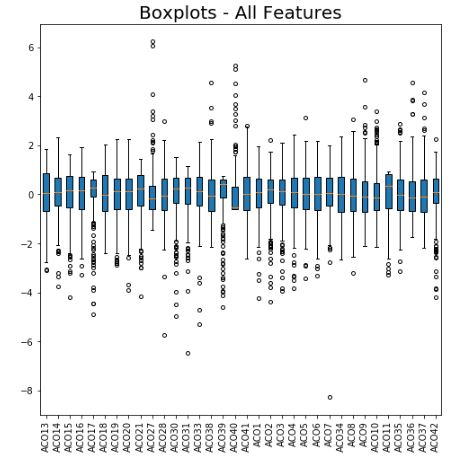
\includegraphics{BoxPlots_ALL.jpg}
    \caption{Boxplot of all features.  Note that the distribution of the features appears to have several anomalous measurements that are quite smaller or larger than their peers.}
    \label{fig:boxall}
\end{figure}
%\todo{RCP: DONE. Maybe that part of the paper should be summarized and some or all of these figures deleted.}
%\todo[color=yellow,inline]{LS:  Add more explanation of analysis of these predictors.  This is the part where we %get to call this a healthcare paper. DONE}

The quality measures can be divided into distinct sub-categories. 
%Boxplots created for each of these categories may reveal differences in the data distributions for each category of features. The GPRO features in particular appear to have greater variability and larger outliers as shown in \ref{fig:boxgpro}.

\begin{enumerate}
\item GPRO - Group Practice Reporting Option Features (18 measures in 7 different groups) : GPRO features are collected by a web interface which was designed specifically to capture ACO-reported clinical quality data.\footnote{The 7 groups are: (1) Care Coordination, (2) Coronary Artery Disease, (3) Heart Failure, (4) Hypertension, (5) Ischemic Vascular Disease, (6) Diabetes, and (7) Method Health and preventive care}

% \begin{figure}[H]
%     \centering
%     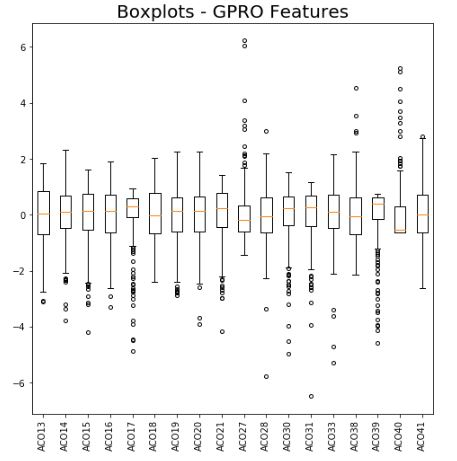
\includegraphics{BoxPlots_GPRO.jpg}
%     \caption{Boxplot of GPRO features}
%     \label{fig:boxgpro}
% \end{figure}


\item CAHPS - Consumer Assessment of Healthcare Providers Survey features (8 measures) : CAHPS features
%LS commented out 24 Jul 2020: , as shown in \ref{fig:boxcahps}, 
are collected by a survey administered by a CMS-approved vendor selected and paid for by individual ACOs. \footnote {The 8 measures are (1) Getting timely care, appointments and information, (2) How well your providers communicate, (3) Patient's rating of provider, (4) Health promotion and education, (6) Shared decision making, (7) Health Status / Functional status, and  (8) Stewardship of patient resources}

% \begin{figure}[H]
%     \centering
%     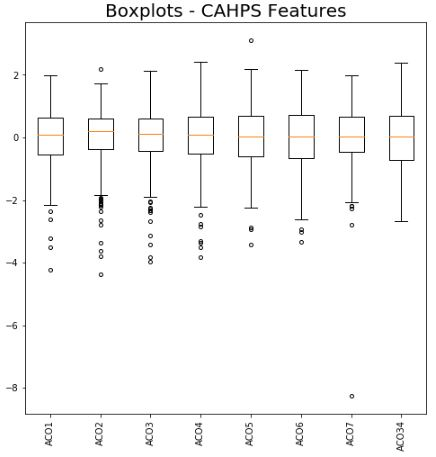
\includegraphics{BoxPlots_CAHPS.jpg}
%     \caption{Boxplot of CAHPS features}
%     \label{fig:boxcahps}
% \end{figure}

\item EHR - Electronic Health Record Features (8 measures): the EHR features is note directly submitted but rather
%LS commented out 24 Jul 2020: ,as shown in Figure \ref{fig:boxehr}, 
 calculated by the CMS ACO PAC based on CMS claims and administrative data extracted from the National Level Repository. \footnote{The 8 measures are 
(1) Risk standardized, All Condition Readmission,
(2) Skilled Nursing Facility 30-Day All-Cause Readmission Measures,
(3) All-Cause Unplanned Admissions for Patients with Diabetes,
(4) All-Cause Unplanned Admissions for Patients with Heart Failure, 
(5) All-Cause Unplanned Admissions for Patients with Multiple Chronic Conditions, 
(6)	Ambulatory Sensitive Conditions Admissions: Chronic Obstructive Pulmonary Disease or Asthma in Older Adults, 
(7) Ambulatory Sensitive Conditions Admissions: Heart Failure,  and 
(8) Percent of Primary Care Physicians who Successfully Meet Meaningful Use Requirements.} 

\end{enumerate}

% \begin{figure}[H]
%     \centering
%     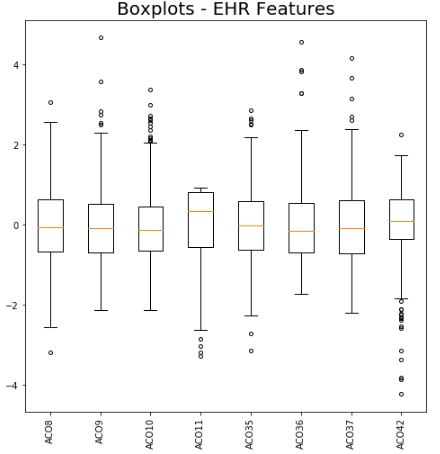
\includegraphics{BoxPlots_EHR.jpg}
%     \caption{Boxplot of EHR features}
%     \label{fig:boxehr}
% \end{figure}



\section{Experimental procedure}
In our experiments we follow the following test protocol to compare the following four competing methods
%\todo[inline]{RCP: I suggest adding an additional sentence of description to each of the methods.  }
\begin{itemize}
    \item Using PCA to make predictions from linear combinations of the original metrics as in Section~\ref{PCA}.
    \item Using SPCA to make predictions from a subset of the original metrics as in Section~\ref{SPCA}.
    \item Perform RPCA first and the use PCA to make predictions from linear combinations of the columns of $L$ as in Section~\ref{PCA}.
    \item Perform RPCA first and the use SPCA to make predictions from a subset of the columns of $L$ as in Section~\ref{SPCA}.
\end{itemize}

Each of these procedures are detailed in the following section.

%TBD TBD TBD TBD TBD TBD TBD TBD TBD TBD TBD TBD TBD TBD TBD TBD TBD TBD TBD TBD TBD TBD TBD TBD TBD TBD TBD TBD TBD TBD TBD TBD TBD TBD TBD TBD TBD TBD TBD TBD.TBD TBD TBD TBD TBD TBD TBD TBD TBD TBD TBD TBD TBD TBD TBD TBD TBD TBD TBD TBD TBD TBD TBD TBD TBD TBD TBD TBD TBD TBD TBD TBD TBD TBD TBD TBD TBD TBD TBD TBD.TBD TBD TBD TBD TBD TBD TBD TBD TBD TBD TBD TBD TBD TBD TBD TBD TBD TBD TBD TBD TBD TBD TBD TBD TBD TBD TBD TBD TBD TBD TBD TBD TBD TBD TBD TBD TBD TBD TBD TBD.

\subsubsection{Pure PCA Approach}

%TBD TBD TBD TBD TBD TBD TBD TBD TBD TBD TBD TBD TBD TBD TBD TBD TBD TBD TBD TBD TBD TBD TBD TBD TBD TBD TBD TBD TBD TBD TBD TBD TBD TBD TBD TBD TBD TBD TBD TBD.TBD TBD TBD TBD TBD TBD TBD TBD TBD TBD TBD TBD TBD TBD TBD TBD TBD TBD TBD TBD TBD TBD TBD TBD TBD TBD TBD TBD TBD TBD TBD TBD TBD TBD TBD TBD TBD TBD TBD TBD.TBD TBD TBD TBD TBD TBD TBD TBD TBD TBD TBD TBD TBD TBD TBD TBD TBD TBD TBD TBD TBD TBD TBD TBD TBD TBD TBD TBD TBD TBD TBD TBD TBD TBD TBD TBD TBD TBD TBD TBD.

%\todo[inline]{RCP: Perhaps these can be combined to make things shorter if we need space.28 Aug: LS doesn't see what is needed with this comment}
%\todo [ color=red,inline]{MITRE wants more detail and/or clarity of the approach for the four approaches}
The pure PCA approach applies Singular Value Decomposition to  the training data set to identify the lower-ranked space according to the number of singular values whose magnitude is larger than some threshold, such as $10^{-3}$.  Reconstruction is performed as described in Section \ref{PCA}. 
%\todo [color = yellow, inline]{Add how it does it,eg "according to the number of singular values strictly above 0 (or should we write "strictly above a specified small positive number")}
%\todo [color = yellow, inline] {Table 1 refers to   the accuracy of reconstructing unmeasured metrics.  Can a sentence be added about how this is done?}
It then projects the test data onto that space and labels the difference between the original test data and the projected data as anomalous as indicated in Algorithm \ref{alg:pca prediction}:
%TBD TBD TBD TBD TBD TBD TBD TBD TBD TBD TBD TBD TBD TBD TBD TBD TBD TBD TBD TBD TBD TBD TBD TBD TBD TBD TBD TBD TBD TBD TBD TBD TBD TBD TBD TBD TBD TBD TBD TBD.TBD TBD TBD TBD TBD TBD TBD TBD TBD TBD TBD TBD TBD TBD TBD TBD TBD TBD TBD TBD TBD TBD TBD TBD TBD TBD TBD TBD TBD TBD TBD TBD

\begin{algorithm}
\caption{PCA prediction}\label{alg:pca prediction}
\begin{algorithmic}[1]
\Procedure{PCA prediction}{$X_{train}, X_{test}$}
\State Perform PCA to get $U \Sigma V^T = SVD(X_{train})$
\State Project $X_{test}$ as $L_{test} = X_{test} V V^T$
\State Anomalies are $S_{test} = X_{test} - L_{test}$
\State \textbf{return} $L_{test}$, $S_{test}$
\EndProcedure
\end{algorithmic}
\end{algorithm}
%\todo [ color = yellow,inline]{ RP: LS added text which should be checked. Also, how does SPCA know how many metrics to select for the pure SPCA approach? For there pure SPCA how does one do reconstruction of unmeasured metrics, cf Table 1?}
%\todo [ color =red, inline]{ Should we change Pure SPCA to "SPCA with PCA" throughout the paper (and patent)?  No, I don't agree with this.  SPCA and PCA are never used together in the paper.}
\subsubsection{SPCA Without RPCA Preprocessing Approach}
The SPCA without RPCA preprocessing, or pure SPCA, approach makes an initial selection of $k$ metrics and selects $k$ columns of the training data and then uses PCA to identify the associated low ranked space.  This space is used to find the low ranked part of the test data and hence the anomalies in the test data. This is formally described in Algorithm \ref{alg:spca prediction}.  Reconstruction is performed as described in Section \ref{SPCA} and the number of metrics is assume to be known \emph{a priori} (a requirement which we can remove when SPCA is combined with RPCA). 
%In detail, the algorithm for our approach is the following when we use SPCA by itself.
% TBD TBD TBD TBD TBD TBD TBD TBD TBD TBD TBD TBD TBD TBD TBD TBD TBD TBD TBD TBD TBD TBD TBD TBD TBD TBD TBD TBD TBD TBD TBD TBD TBD TBD TBD TBD TBD TBD TBD TBD.TBD TBD TBD TBD TBD TBD TBD TBD TBD TBD TBD TBD TBD TBD TBD TBD TBD TBD TBD TBD TBD TBD TBD TBD TBD TBD TBD TBD TBD TBD TBD TBD
%\todo [ color = red,inline]{Why isn't Algorithm 2 listed here? DONE}
\begin{algorithm}
\caption{SPCA prediction}\label{alg:spca prediction}
\begin{algorithmic}[1]
\Procedure{SPCA prediction}{$X_{train}, X_{test}$}
\State Make a selection matrix $\mathfrak{S}_{sel}$
\State Select $k$ columns of $X_{train}$ to get $X_k = X_{train} \mathfrak{S}_{sel}$
\State Perform PCA to get $U \Sigma V^T = SVD(X_k)$
%new
\State Set $Z = X_k (\mathfrak{S}_{sel}^T - \mathfrak{S}_{sel}^T V V^T)  ((I-\mathfrak{S}_{sel} \mathfrak{S}_{sel}^T)V V^T - (I-\mathfrak{S}_{sel} \mathfrak{S}_{sel}^T))^{-1}$
%end of new
%\State Solve for $Z$ using $X_k (\mathfrak{S}_{sel}^T - \mathfrak{S}_{sel}^T V V^T) = Z ((I-\mathfrak{S}_{sel} \mathfrak{S}_{sel}^T)V V^T - (I-\mathfrak{S}_{sel} \mathfrak{S}_{sel}^T))$.
\State Project $X_{test}$ as $L_{test} = X_{test} \mathfrak{S}_{sel} \mathfrak{S}_{sel}^T + Z (I-\mathfrak{S}_{sel} \mathfrak{S}_{sel}^T)$.
\State Anomalies are $S_{test} = X_{test} - L_{test}$
\State \textbf{return} $L_{test}$, $S_{test}$
\EndProcedure
\end{algorithmic}
\end{algorithm}

%\todo[inline]{RCP:  Make clear what projectx-test is.  Can use new notation in Traditional PCA section.28 Aug: LS doesn't understand this comment}
%\todo [inline,color = yellow] {Table 1 refers to the accuracy of reconstructing unmeasured metrics.  How is this done with this method?}
\subsubsection{PCA with RPCA Preprocessing Approach}
%In detail, the algorithm for our approach is the following when we use PCA by after RPCA preprocessing. 
Here RPCA is applied to the training data to identify the low ranked space of the training data.  Next, PCA is applied to the projection of the test data onto that space to identify the low rank test data and the anomalies in the test data.  The RPCA preprocessing step prevents the anomalies in the training data from inducing incorrect errors when processing the test data.  This is formally described in Algorithm \ref{alg:pca and rpca prediction}.
% TBD TBD TBD TBD TBD TBD TBD TBD TBD TBD TBD TBD TBD TBD TBD TBD TBD TBD TBD TBD TBD TBD TBD TBD TBD TBD TBD TBD TBD TBD TBD TBD TBD TBD TBD TBD TBD TBD TBD TBD.TBD TBD TBD TBD TBD TBD TBD TBD TBD TBD TBD TBD TBD TBD TBD TBD TBD TBD TBD TBD TBD TBD TBD TBD TBD TBD TBD TBD TBD TBD TBD TBD

\begin{algorithm}
\caption{PCA prediction with RPCA preprocessing}\label{alg:pca and rpca prediction}
\begin{algorithmic}[1]
\Procedure{PCA prediction}{$X_{train}, X_{test}$}
\State Perform RPCA to get $L_{train}, S_{train} = RPCA(X_{train})$
\State Perform PCA to get $U \Sigma V^T = SVD(L_{train})$
\State Project $X_{test}$ as $L_{test} = X_{test} V V^T$
\State Anomalies are $S_{test} = X_{test} - L_{test}$
\State \textbf{return} $L_{test}$, $S_{test}$
\EndProcedure
\end{algorithmic}
\end{algorithm}
\subsubsection{SPCA with RPCA Preprocessing Approach}
In a manner similar to the  PCA with RPCA preprocessing approach, this approach applies RPCA to the SPCA analysis of the training data to prevent the anomalies in the training data from inducing incorrect errors when processing the test data.  This is formally described in Algorithm \ref {alg:spca and rpca prediction}.
%In detail, the algorithm for our approach is the following when we use SPCA by after RPCA preprocessing. 
%TBD TBD TBD TBD TBD TBD TBD TBD TBD TBD TBD TBD TBD TBD TBD TBD TBD TBD TBD TBD TBD TBD TBD TBD TBD TBD TBD TBD TBD TBD TBD TBD TBD TBD TBD TBD TBD TBD TBD TBD.TBD TBD TBD TBD TBD TBD TBD TBD TBD TBD TBD TBD TBD TBD TBD TBD TBD TBD TBD TBD TBD TBD TBD TBD TBD TBD TBD TBD TBD TBD TBD TBD

\begin{algorithm}
\caption{SPCA prediction with RPCA preprocessing}\label{alg:spca and rpca prediction}
\begin{algorithmic}[1]
\Procedure{SPCA prediction}{$X_{train}, X_{test}$}
\State Perform RPCA to get $L_{train}, S_{train} = RPCA(X_{train})$
\State Make a selection matrix $\mathfrak{S}_{sel}$
\State Select $k$ columns of $L_{train}$ to get $L_k = L_{train} \mathfrak{S}_{sel}$
\State Perform PCA to get $U \Sigma V^T = SVD(L_k)$
% We Should just do it:\State Solve for $Z$ using $L_k (\mathfrak{S}_{sel}^T - \mathfrak{S}_{sel}^T V V^T) = Z ((I-\mathfrak{S}_{sel} \mathfrak{S}_{sel}^T)V V^T - (I-\mathfrak{S}_{sel} \mathfrak{S}_{sel}^T))$.
\State Set $Z = L_k (\mathfrak{S}_{sel}^T - \mathfrak{S}_{sel}^T V V^T) ((I-\mathfrak{S}_{sel} \mathfrak{S}_{sel}^T)V V^T - (I-\mathfrak{S}_{sel} \mathfrak{S}_{sel}^T))^{-1}$.
\State Project $X_{test}$ as $L_{test} = X_{test} \mathfrak{S}_{sel} \mathfrak{S}_{sel}^T + Z (I-\mathfrak{S}_{sel} \mathfrak{S}_{sel}^T)$.
\State Anomalies are $S_{test} = X_{test} - L_{test}$
\State \textbf{return} $L_{test}$, $S_{test}$
\EndProcedure
\end{algorithmic}
\end{algorithm}
%\todo [color = yellow,inline] {Should we also return Z in algorithm 4?28 AUg: I think I wrote this comment but no longer understand it}
% \begin{enumerate}
% \item Create data with rank 6 where we know precisely the relationships between all columns
% \item Insert outliers
% \item Split matrix X into XTrain/XTest
% \item Normalize each column of the training set
% \item Set a threshold to flag values in S as outliers when running RPCA
% \item Run RPCA iteratively with different $\lambda$ values until the expected number of anomalies appear in S
% \item Generate L, S
% \item Unnormalize L to return data to original scale
% \item Compute $\alpha$ in $A\alpha = B$ in the training set for each column, resulting in 14 vectors of length 6 (one for each column), explaining the relationship between the first 6 columns and the column in question
% \item User the first 6 columns of the XTest and $\alpha$ to predict columns 7-20
% \item Compute MSE of predictions only on points which are truly not outliers
% \end{enumerate}

\section{Results}
\label{results}
%\todo [ color = orange,inline] {RP: LS asks: For Table 1 does the rank estimate refer to the case of no anomalies or the case of anomalies?}
%\todo[inline]{Need to talk about training and testing setup better.}
%\todo [ color = red]{ RP: MITRE ask: He doesn't like the "??"in the table. LS changed to na.  RP: OK?}
The following results demonstrate a comparison of traditional methods and Robust Principal Components Analysis performed on synthetic data with noise and varying amounts and sizes of anomalies added.  As we will detail below, Figures \ref{fig:m_200_n_20_k_6_numAnoms_10_sizeAnoms_0.001000} through \ref{fig:real_data}
%\todo [ color = yellow, inline]{ By plot do you mean one of the figures.  Perhaps we should state FIgure x - y reveal that ...}
demonstrate that combining RPCA and SPCA provides the ability to detect the true rank of the data (which was created to be of rank-6) and accurately unmeasured reconstruct metrics, while competing methods, such as PCA, have trouble detecting the rank are thrown off by noise and anamolies.  Additional evidence is provided in the confusion matrix plots which show a significantly better False Positive rate using the RPCA method.
%\todo[inline]{RCP: Should state why it is useful that we are getting the true rank. btw, is this causing the confusion matrix to be better or is it also true that the confusion matrix is better}

In this paper we present several different types of results and Table \ref{tab:table1} compares the various techniques we have explored. For these experiments synthetic data is generated with $20$ interdependent metrics having a true rank of $6$.  $100$ rows are generated for training the PCA, SPCA and RPCA algorithms, as described in Algorithms \ref{alg:pca prediction} through \ref{alg:spca and rpca prediction}, and $100$ additional rows are generated for testing the various combinations of methods.   In both the training and testing data we introduce $5$ anomalies of size $1$.  For comparison purposes the nominal data entries range in size from close to $0$ to around $10$, so the anomalies are are order of magnitude smaller than some normal entries.
In particular, the methods that use RPCA preprocessing correctly detect that the true rank is $6$, even in the presence of anomalies, while the PCA method incorrectly estimates the rank to be $9$ because of the anomalies.  SPCA does not, inherently, provide an estimate of the rank so in our experiments it was either provided with the true rank or, when combined with RPCA, uses the rank estimate provided by the RPCA algorithm.  Also, when SPCA is used with RPCA, the columns that SPCA chooses are columns that RPCA identifies as anomaly free in the training data. \footnote{Note that in Table \ref{tab:table1} we focus on recovery of non-anomalous entries.  Recovery of anomalous entries in testing data is not a reasonable goal.}
%\todo[inline]{RCP:  Create table to summarize Fig 5-8.  28 Aug 2020: THis was an old suggestion.  I assume this is Table 1 and table 2.  Is there any other synthesis of results which is possible?  (I assume the answer is no but wanted to confirm}
%\todo [inline]{I still don't understand precisely what the follow table is measuring: is the reconstruction on the first line assuming 9 composite measures are used?  How is SPCA doing any reconstruction without PCA or RPCA going first. What does PCA with RPCA mean? RP: Would you please add a few more words?}
\begin{table}[h!]
    \begin{center}
      \caption{RMSE error of reconstructions.}
      \label{tab:table1}
      \begin{tabular}{l|c|c|c} % <-- Alignments: 1st column left, 2nd middle and 3rd right, with vertical lines in between
        \textbf{Reconstruction type} & \textbf{Rank} & \begin{minipage}{0.42in}\textbf{\# metrics  to measure}\end{minipage}  & \begin{minipage}{0.50in}\textbf{RMSE with no anomaly in testing}\end{minipage} \\
        \hline
        PCA & 9 & 20 & 4.3e-1 \\
        SPCA &N/A & 6 & 2.3e0 \\
        PCA with RPCA & 6 & 20 & 5.3e-4 \\
        SPCA with RPCA & 6 & 6 & 2.7e-3 \\
      \end{tabular}
    \end{center}
\end{table}
% \begin{table}[h!]
%     \begin{center}
%       \caption{RMSE error of reconstructions.}
%       \label{tab:table1}
%       \begin{tabular}{l|c|c|c|c} % <-- Alignments: 1st column left, 2nd middle and 3rd right, with vertical lines in between
%         \textbf{Reconstruction type} & \textbf{Rank} & \begin{minipage}{0.42in}\textbf{\# metrics  to measure}\end{minipage}  & \begin{minipage}{0.50in}\textbf{RMSE with no anomaly in testing}\end{minipage} & \begin{minipage}{0.50in}\textbf{RMSE with anomaly in testing}\end{minipage}\\
%         \hline
%         PCA & 9 & 20 & 4.3e-1 & 1.3e0\\
%         SPCA &N/A & 6 & 2.3e0 & 4.7e0 \\
%         PCA with RPCA & 6 & 20 & 5.3e-4 & 1.8e0  \\
%         SPCA with RPCA & 6 & 6 & 2.7e-3 & 6.3e0 \\
%       \end{tabular}
%     \end{center}
% \end{table}
\noindent

Table \ref{tab:table2} compares the F1 score\footnote{Formally, the F1 Score is the harmonic mean of the \emph{precision} and the \emph{recall}.  The  \emph{precision} is  the number of true positive results divided by the number of true positives plus the number of false positive. The \emph{recall} is the number of true positives divided by the number of true positives plus the number of false negatives.} of the four approaches for detecting anomalies.  The F1-score balances false-positives and false-negatives.  The best possible score is $1$ and the worst possible score is $0$.  The PCA and SPCA algorithms perform quite badly both because of anomalies in the training data and the anomalies in the testing data.  However, in the presence of RPCA preprocessing, both the PCA and SPCA algorithms perform quite well.  However, as our focus is on reducing the reporting burden on healthcare providers, only the SPCA algorithm combined with RPCA preprocessing provides all of the capabitilies that we require. 
\begin{table}[h!]
    \begin{center}
      \caption{F1-score for anomaly detection. }
      \label{tab:table2}
      \begin{tabular}{l|c} % <-- Alignments: 1st column left, 2nd middle and 3rd right, with vertical lines in between
        \textbf{Reconstruction type} & \begin{minipage}{1in}\textbf{F1-score for anomaly detection}\end{minipage}\\
        \hline
        PCA &  0.23 \\
        SPCA &  0.51 \\
        PCA with RPCA &  0.97 \\
        SPCA with RPCA &  0.99 \\
      \end{tabular}
    \end{center}
\end{table}

%\todo[color = orange,inline]{RCP: LS added a lot of words in the following paragraph to explain the figures.  It would be nice if RP checked this}
%\todo [ color = red,inline]{RP: SHould we eliminate some subset of Fig 2-6 to save space?DONE}
%\todo [ color = red,inline] {RP: I took the number of anomalies you listed in the legend and divided by 2 because RPCA was applied to a single data set: the test setOLD NEWS}
In Figures~\ref{fig:m_200_n_20_k_6_numAnoms_10_sizeAnoms_0.001000}, \ref{fig:m_200_n_20_k_6_numAnoms_10_sizeAnoms_1.000000}, and
\ref{fig:difficult RPCA} we show the performance of the RPCA algorithm running alone across a variety of scenarios. 
% \todo[inline]{RCP:  Be sure to talk about the $\lambda$ values that are chosen for each figure.}
% \todo [inline, color = red]{28 Aug: LS ran out of steam here so rest not checked carefully}
Figure \ref{fig:m_200_n_20_k_6_numAnoms_10_sizeAnoms_0.001000} shows the results of RPCA running alone in the presence of very small anomalies.   In this parameter range using RPCA alone has difficulty detecting the anomalies since they are three orders of magnitude smaller than the ambient low-rank background.  As a result, the flagged anomalies, displayed in the fourth graphic, are not displayed in the third graphic of true anomalies. This indicates that there are many falsely detected anomalies.
%\todo [color = orange,inline] {RP: LS thinks Figure 6 should be split into two (maybe four) figures and more words should be added to the rank part of the discussion in the text here}
%\todo [ color = red,inline] {RCP:Fix reference error}
Figure \ref{fig:m_200_n_20_k_6_numAnoms_10_sizeAnoms_1.000000} shows RPCA running alone on data with a small number of anomalies of the same order of magnitude as the low-rank background.  By comparing the third and fourth graphics one sees that in this parameter regime, the RPCA algorithm alone can easily detect the true anomalies and has no false detections.  
% Figure \ref{fig:m_200_n_20_k_6_numAnoms_10_sizeAnoms_50.000000} shows some very large anomalies, and again running the RPCA algorithm alone performs perfectly. 
% Figure \ref {fig:m_200_n_20_k_6_numAnoms_50_sizeAnoms_0.010000} displays a hard example with many small anomalies yet running RPCA alone does a good job.
Figure \ref{fig:difficult RPCA} shows the limits of the RPCA algorithm in the presence of many anomalies.   On the left, the rank is computed correctly, but on the right the problem is so difficult that the rank is computed incorrectly as well.
In particular, the idea of training the RPCA algorithm is to choose a $\lambda$ value, as in (\ref{mainalg}), with two properties on the training data.  First, and most importantly, the $\lambda$ value should recover the correct rank.  Accordingly, as in Figure \ref{fig:difficult RPCA}, the $\lambda$ value chosen for the first graphic would be an appropriate choice.  Second, if a range of $\lambda$ values were to all recover the correct rank then the choosing a $\lambda$ value in this range that minimizes the number of false-positives and false-negatives in detecting the anomalies in $S$ would lead to the most effective algorithm.
 
% \todo [color = orange,inline] {Would be nice to clarify the rank discussion}
%\todo [color = red,inline]{Figure 5 has a typo in the graphic traing --> training so I cannot fix it}
% Insert Figures for three percent anomalies size 5

\begin{figure}
    \begin{subfigure}{.45\textwidth}
    \centering
    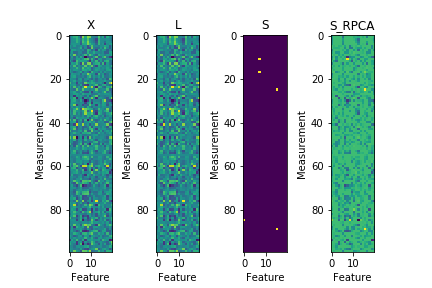
\includegraphics[width=.9\linewidth]{{images/new_7-26-2020/runRPCAAnomalyTest_images_m_200_n_20_k_6_numAnoms_10_sizeAnoms_0.001000}.png}
    \end{subfigure}
    % \begin{subfigure}{.45\textwidth}
    % \centering
    % 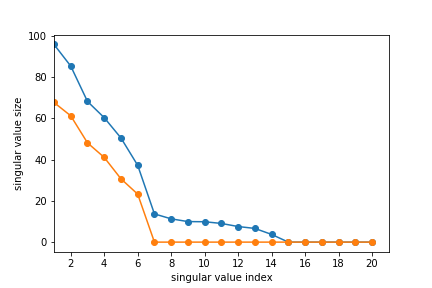
\includegraphics[width=.9\linewidth]{{images/new_7-26-2020/runRPCAAnomalyTest_singular_values_m_200_n_20_k_6_numAnoms_10_sizeAnoms_0.001000}.png}
    % \end{subfigure}
    \caption{A difficult example of RPCA with $5$ anomalies  each of size $0.001$.  The original $X$ matrix and computed $L$ matrix are shown in the first two Figures. The fourth Figure (with title S\_RPCA) shows the anomalies detected by the RPCA algorithm, and it is quite different than the third Figure (with title S) which shows the true anomalies.}
    \label{fig:m_200_n_20_k_6_numAnoms_10_sizeAnoms_0.001000}
\end{figure}

%\todo[inline]{RCP: The labels for fig 5-8 should all be different.  Are they all needed: SHoudl we only included the hardest case it does well on and the simplest one it doesn't poorly on?  Also, the blue and orange curves are incorrect (code error) and need legends and better titles.}

\begin{figure}
    \begin{subfigure}{.45\textwidth}
    \centering
    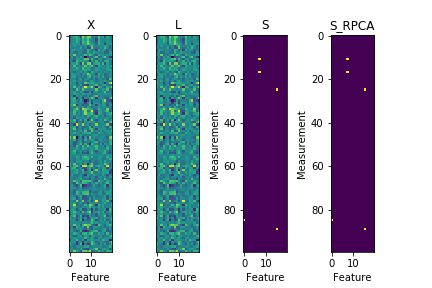
\includegraphics[width=.9\linewidth]{{images/new_7-26-2020/runRPCAAnomalyTest_images_m_200_n_20_k_6_numAnoms_10_sizeAnoms_1.000000}.png}
    \end{subfigure}
    % \begin{subfigure}{.45\textwidth}
    % \centering
    % 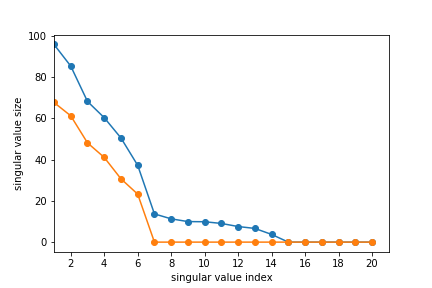
\includegraphics[width=.9\linewidth]{{images/new_7-26-2020/runRPCAAnomalyTest_singular_values_m_200_n_20_k_6_numAnoms_10_sizeAnoms_1.000000}.png}
    % \end{subfigure}
    \caption{An easy example of RPCA with $5$ anomalies each of size $1$. The third and fourth Figures and nearly identical demonstrating that the RPCA algorithm has successfully detected all anomalies. }
    \label{fig:m_200_n_20_k_6_numAnoms_10_sizeAnoms_1.000000}
\end{figure}

% \begin{figure}
%     \begin{subfigure}{.45\textwidth}
%     \centering
%     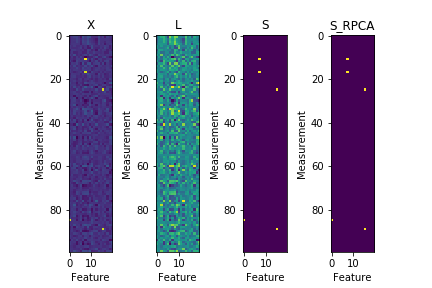
\includegraphics[width=.9\linewidth]{{images/new_7-26-2020/runRPCAAnomalyTest_images_m_200_n_20_k_6_numAnoms_10_sizeAnoms_50.000000}.png}
%     \end{subfigure}
%     % \begin{subfigure}{.45\textwidth}
%     % \centering
%     % 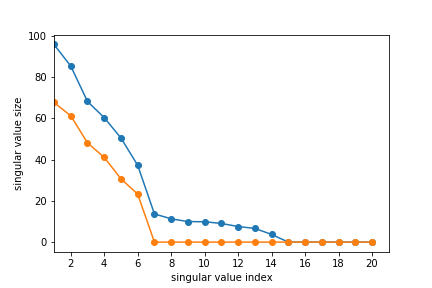
\includegraphics[width=.9\linewidth]{{images/new_7-26-2020/runRPCAAnomalyTest_singular_values_m_200_n_20_k_6_numAnoms_10_sizeAnoms_50.000000}.png}
%     % \end{subfigure}
%     \caption{An easy example of RPCA with $5$ anomalies each of size $50$.}
%     \label{fig:m_200_n_20_k_6_numAnoms_10_sizeAnoms_50.000000}
% \end{figure}

% \begin{figure}
%     \begin{subfigure}{.45\textwidth}
%     \centering
%     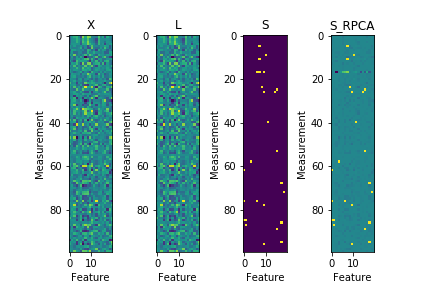
\includegraphics[width=.9\linewidth]{{images/new_7-26-2020/runRPCAAnomalyTest_images_m_200_n_20_k_6_numAnoms_50_sizeAnoms_0.010000}.png}
%     \end{subfigure}
%     % \begin{subfigure}{.45\textwidth}
%     % \centering
%     % 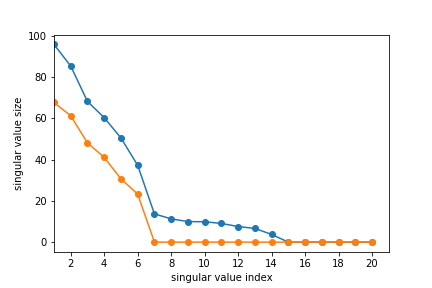
\includegraphics[width=.9\linewidth]{{images/new_7-26-2020/runRPCAAnomalyTest_singular_values_m_200_n_20_k_6_numAnoms_50_sizeAnoms_0.010000}.png}
%     % \end{subfigure}
%     \caption{A difficult example of RPCA with $50$ anomalies, each of size $0.01$.  }
%     \label{fig:m_200_n_20_k_6_numAnoms_50_sizeAnoms_0.010000}
% \end{figure}

\begin{figure*}
    \centering
    \begin{subfigure}{.45\textwidth}
    \centering
    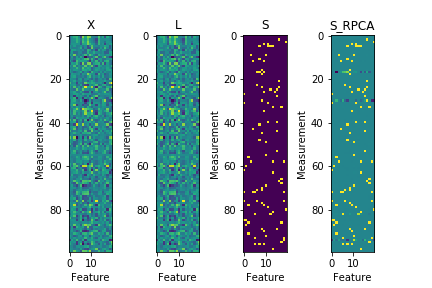
\includegraphics[width=.9\linewidth]{{images/new_7-26-2020/runRPCAAnomalyTest_images_m_200_n_20_k_6_numAnoms_200_sizeAnoms_0.100000}.png}
    \end{subfigure}
    \begin{subfigure}{.45\textwidth}
    \centering
    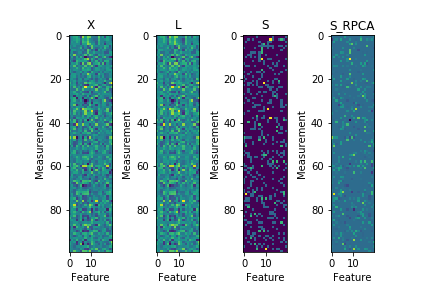
\includegraphics[width=.9\linewidth]{{images/new_7-26-2020/runRPCAAnomalyTest_images_m_200_n_20_k_6_numAnoms_1000_sizeAnoms_1.000000}.png}
    \end{subfigure}

    \begin{subfigure}{.45\textwidth}
    \centering
    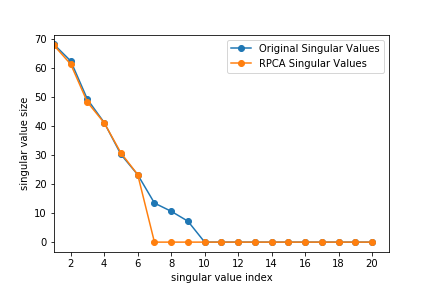
\includegraphics[width=.9\linewidth]{{images/new_7-26-2020/runRPCAAnomalyTest_singular_values_m_200_n_20_k_6_numAnoms_200_sizeAnoms_0.100000}.png}
    \end{subfigure} 
    \begin{subfigure}{.45\textwidth}
    \centering
    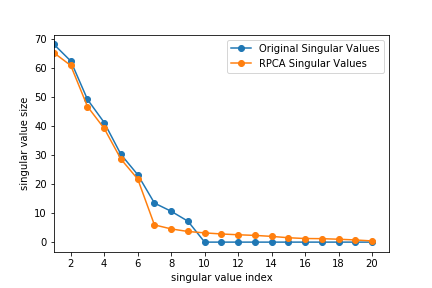
\includegraphics[width=.9\linewidth]{{images/new_7-26-2020/runRPCAAnomalyTest_singular_values_m_200_n_20_k_6_numAnoms_1000_sizeAnoms_1.000000}.png}
    \end{subfigure}

    \caption{A difficult example of RPCA with $50$ anomalies  each of size $0.1$ on the left and $500$ anomalies, each of size $1$ on the right. }
    \label{fig:difficult RPCA}
\end{figure*}

%%%%%%%%%%%%%%%%%%%%%%%%%%%%%%%%%%%%%%%%%%%%%%%%%%%%%%%%%%%%%%%%
%\todo [ color = orange,inline] {RP: I would like a better understanding of these figures and then LS would be glad to add text to them, e.g. what was the experiment performed}
The key results of our work can be found in Figures \ref{fig:error_PCA_prediction_without_RPCA} -  
%\ref{fig:error_PCA_prediction_with_RPCA_first}, \ref{fig:error_SPCA_prediction_without_RPCA_first}, \ref{fig:error_SPCA_prediction_without_RPCA_first_selected}, \ref{fig:error_SPCA_prediction_with_RPCA_first}, and 
\ref{fig:error_SPCA_prediction_with_RPCA_first_selected}.
Figure \ref{fig:error_PCA_prediction_without_RPCA} shows a purely PCA based prediction.  Besides requiring all of the original metrics to compute, the anomalies in the training and testing data cause many errors in reconstruction in both the rows and the columns.  The errors in the columns are caused by anomalies in the training data set which are unknown to the PCA algorithm and therefore are induced into errors in the test data reconstruction.  The errors in the rows are caused be anomalies in the test data which are unknown to the PCA algorithm and therefore used to incorrectly reconstruct the test data.  %These errors are unavoidable so in Figure \ref {fig:error_PCA_prediction_without_RPCA} those rows are not displayed in Figure \ref {fig:error_PCA_prediction_without_RPCA_selected}.
%\todo [ color = red] {RP: Delete figure 8 to save space?  Should we add another figure above Fig7 to show how the anomalies in the training data corrupts predictions in the test data.}
% Similarly, Figures \ref{fig:error_PCA_prediction_with_RPCA_first}  and  \ref {fig:error_PCA_prediction_with_RPCA_first_selected} shows how processing the training data with RPCA eliminates the reconstruction errors in some columns leaving only unavoidable reconstruction errors in rows of the test data with anomalies.   

Figure \ref{fig:error_SPCA_prediction_without_RPCA_first_selected} shows a SPCA prediction without PRCA processing.  Again, reconstruction errors are found in columns caused by anomalies in the training data and rows if there are anomalies in the training data metrics which were used.  Note that SPCA, unlike PCA, uses only some of the metrics in the test data for reconstruction, which are illustrated in green. The use of a subset reduces induced reconstruction errors.
%after an RPCA preprocessing.  While superior to the pure PCA reconstruction, anomalies in the testing data still cause substantial errors. 
%\todo[color=yellow]{LS: It seems that Fig 14 and 15 are the big achievement: Some in a quantitative form this should be summarized in the intro}
Finally, Figure \ref{fig:error_SPCA_prediction_with_RPCA_first_selected} shows an SPCA prediction after an RPCA preprocessing.  In this case both the low-rank background and the anomalies are exactly recovered, up to the error arising in the RPCA optimization, for the rows of the test data which do not use anomalous metrics (shown in green).

\begin{figure}
    \centering
    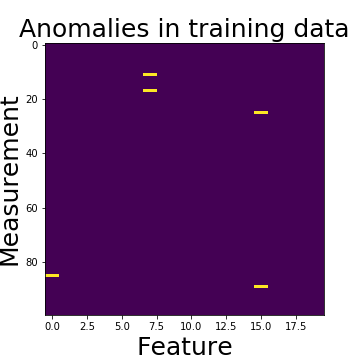
\includegraphics[width=0.24\textwidth]{{images/new_8-31-2020/short_test_S_title_PCA_prediction_without_RPCA_first_m_200_n_20_k_6_noiseSize_0.000000_numAnoms_10_sizeAnoms_1.000000_train}.png}
    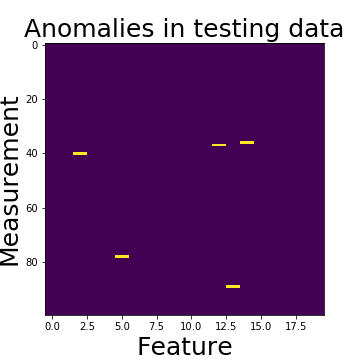
\includegraphics[width=0.24\textwidth]{{images/new_8-31-2020/short_test_S_title_PCA_prediction_without_RPCA_first_m_200_n_20_k_6_noiseSize_0.000000_numAnoms_10_sizeAnoms_1.000000_left}.png}\\
    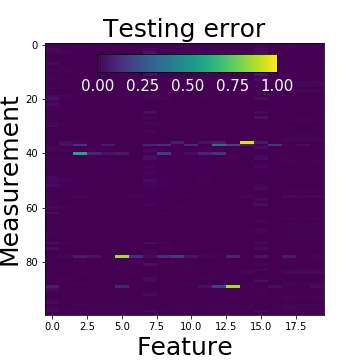
\includegraphics[width=0.24\textwidth]{{images/new_8-31-2020/short_test_S_title_PCA_prediction_without_RPCA_first_m_200_n_20_k_6_noiseSize_0.000000_numAnoms_10_sizeAnoms_1.000000_right}.png}
\caption{A PCA prediction without RPCA first.  The top left shows the anomalies in the training data, and the top right shows the anomalies in the testing data.  The errors in the bottom are a function of both types of errors, with errors in whole rows arising from the errors in the testing data.
%Note that both columns and rows have noise.
}
\label{fig:error_PCA_prediction_without_RPCA}
\end{figure}

% \begin{figure}
%     \centering
%     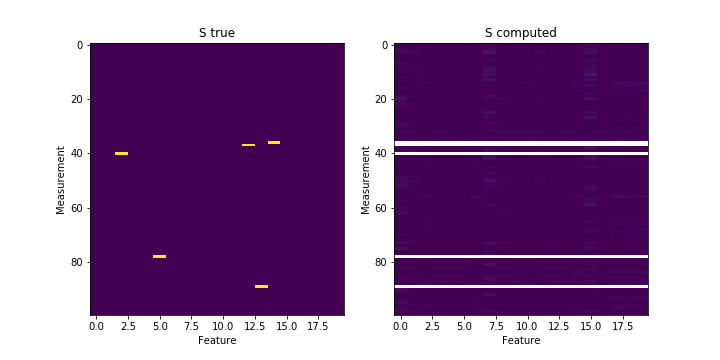
\includegraphics[width=0.45\textwidth]{{images/new_7-26-2020/short_test_S_title_PCA_prediction_without_RPCA_first_selected_m_200_n_20_k_6_noiseSize_0.000000_numAnoms_10_sizeAnoms_1.000000}.png}
%     \caption{A PCA prediction without RPCA first.  
%     %Note that both columns and rows have noise. 
%     In this figure we emphasize the errors caused by test data  anomalies by removing those rows.
%     }
%   \label{fig:error_PCA_prediction_without_RPCA_selected}
% \end{figure}


% \begin{figure}
%     \centering
%     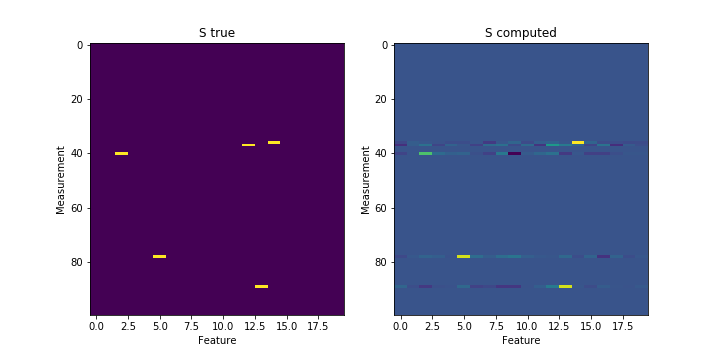
\includegraphics[width=0.45\textwidth]{{images/new_7-26-2020/short_test_S_title_PCA_prediction_with_RPCA_first_m_200_n_20_k_6_noiseSize_0.000000_numAnoms_10_sizeAnoms_1.000000}.png}
%     \caption{A PCA prediction with RPCA first. 
%     %Note that only the rows have noise where there are anomalies in the testing data.
%     }
%     \label{fig:error_PCA_prediction_with_RPCA_first}
% \end{figure}

% \begin{figure}
%     \centering
%     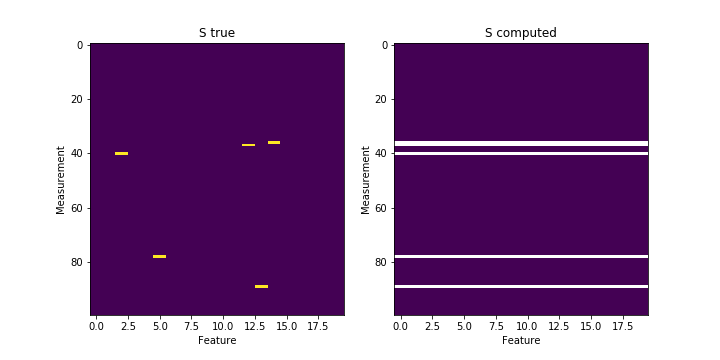
\includegraphics[width=0.45\textwidth]{{images/new_7-26-2020/short_test_S_title_PCA_prediction_with_RPCA_first_selected_m_200_n_20_k_6_noiseSize_0.000000_numAnoms_10_sizeAnoms_1.000000}.png}
%     \caption{A PCA prediction with RPCA first. 
%     %Note that only the rows have noise where there are anomalies in the testing data.  
%     In this figure we emphasize the errors caused by training data by removing the rows with anomalies in the testing data.
%     }
%     \label{fig:error_PCA_prediction_with_RPCA_first_selected}
% \end{figure}


\begin{figure}
\centering
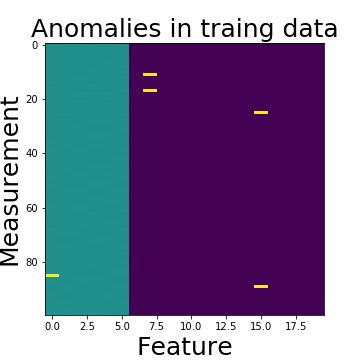
\includegraphics[width=0.24\textwidth]{{images/new_8-31-2020/short_test_S_title_SPCA_prediction_without_RPCA_first_m_200_n_20_k_6_noiseSize_0.000000_numAnoms_10_sizeAnoms_1.000000_train}.png}
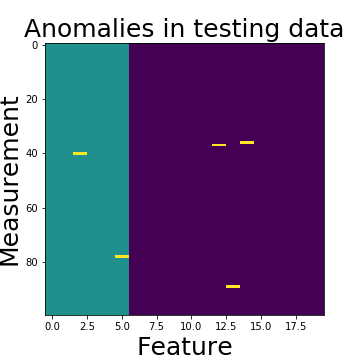
\includegraphics[width=0.24\textwidth]{{images/new_8-31-2020/short_test_S_title_SPCA_prediction_without_RPCA_first_m_200_n_20_k_6_noiseSize_0.000000_numAnoms_10_sizeAnoms_1.000000_left}.png}
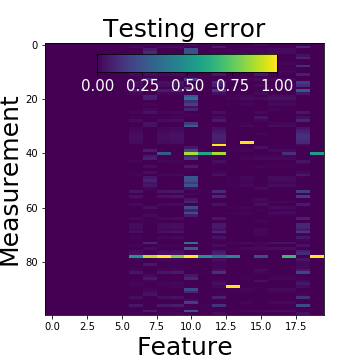
\includegraphics[width=0.24\textwidth]{{images/new_8-31-2020/short_test_S_title_SPCA_prediction_without_RPCA_first_m_200_n_20_k_6_noiseSize_0.000000_numAnoms_10_sizeAnoms_1.000000_right}.png}
%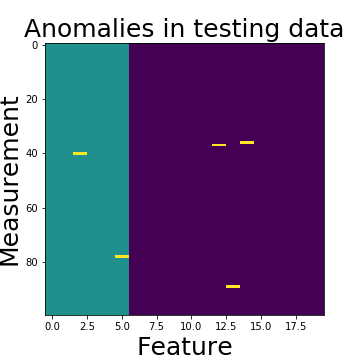
\includegraphics[width=0.24\textwidth]{{images/new_8-5-2020/short_test_S_title_SPCA_prediction_without_RPCA_first_selected_m_200_n_20_k_6_noiseSize_0.000000_numAnoms_10_sizeAnoms_1.000000_left}.png}
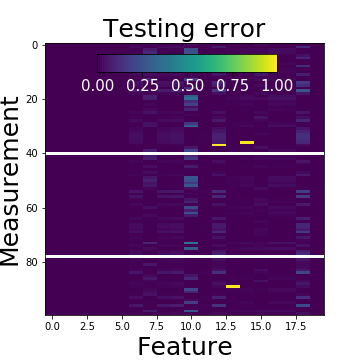
\includegraphics[width=0.24\textwidth]{{images/new_8-31-2020/short_test_S_title_SPCA_prediction_without_RPCA_first_selected_m_200_n_20_k_6_noiseSize_0.000000_numAnoms_10_sizeAnoms_1.000000_right}.png}
\caption{An SPCA prediction without RPCA first.  
The top left shows the anomalies in the training data, and the top right shows the anomalies in the testing data.  The green columns are those columns that are used to reconstruct the rest.  The bottom two figures show the errors in the reconstruction. As there is an anomaly in the green columns in the training data, that one anomaly leads to inaccuracies in many predictions in the testing data, which we emphasize in the bottom right figure by removing the rows which have error arising from anomalies in the testing data.}
\label{fig:error_SPCA_prediction_without_RPCA_first_selected}
\end{figure}


% \begin{figure*}
% \begin{subfigure}{.45\textwidth}
%     \centering
%     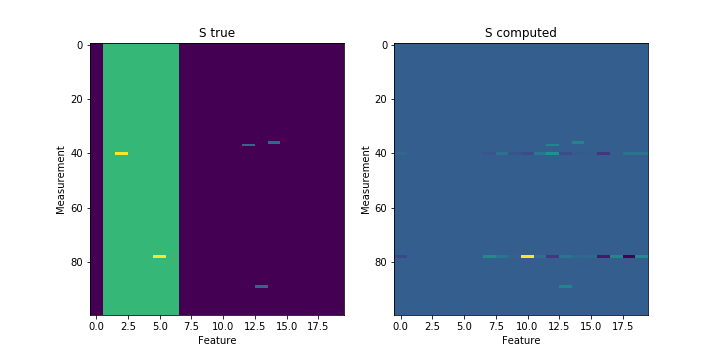
\includegraphics[width=0.9\textwidth]{{images/new_7-26-2020/short_test_S_title_SPCA_prediction_with_RPCA_first_m_200_n_20_k_6_noiseSize_0.000000_numAnoms_10_sizeAnoms_1.000000}.png}
%     \caption{An SPCA prediction without RPCA first.  
%Note that, similar to PCA with RPCA, both only rows are incorrect because of anomalies in the testing data.
%}
%     \label{fig:error_SPCA_prediction_with_RPCA_first}
% \end{subfigure}
% \begin{subfigure}{.45\textwidth}
%     \centering
%     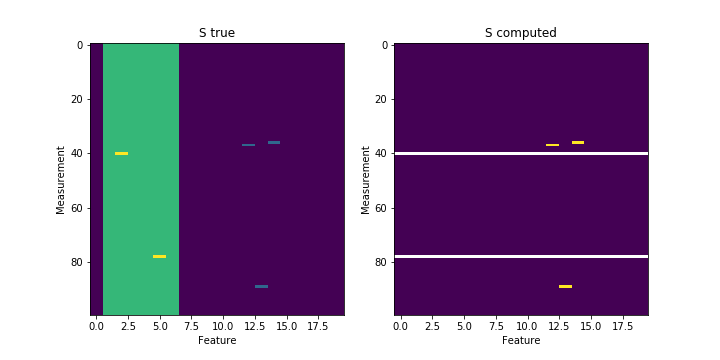
\includegraphics[width=0.9\textwidth]{{images/new_7-26-2020/short_test_S_title_SPCA_prediction_with_RPCA_first_selected_m_200_n_20_k_6_noiseSize_0.000000_numAnoms_10_sizeAnoms_1.000000}.png}
%     \caption{An SPCA prediction without RPCA first.  Note that, similar to PCA with RPCA, both only rows are incorrect because of anomalies in the testing data.  In this figure we show that the anomalies are exactly recovered in by removing the rows with anomalies in the testing data.}
%     \label{fig:error_SPCA_prediction_with_RPCA_first_selected}
% \end{subfigure}
% \end{figure*}

\begin{figure}
\centering
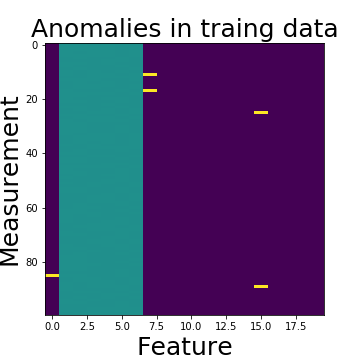
\includegraphics[width=0.24\textwidth]{{images/new_8-31-2020/short_test_S_title_SPCA_prediction_with_RPCA_first_m_200_n_20_k_6_noiseSize_0.000000_numAnoms_10_sizeAnoms_1.000000_train}.png}
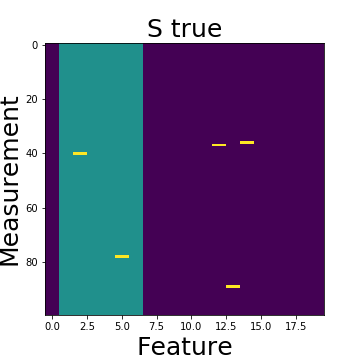
\includegraphics[width=0.24\textwidth]{{images/new_8-31-2020/short_test_S_title_SPCA_prediction_with_RPCA_first_m_200_n_20_k_6_noiseSize_0.000000_numAnoms_10_sizeAnoms_1.000000_left}.png}
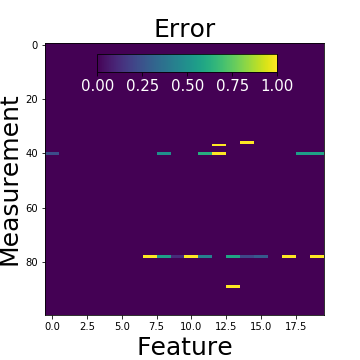
\includegraphics[width=0.24\textwidth]{{images/new_8-31-2020/short_test_S_title_SPCA_prediction_with_RPCA_first_m_200_n_20_k_6_noiseSize_0.000000_numAnoms_10_sizeAnoms_1.000000_right}.png}
%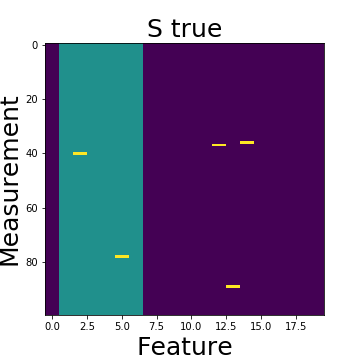
\includegraphics[width=0.24\textwidth]{{images/new_8-5-2020/short_test_S_title_SPCA_prediction_with_RPCA_first_selected_m_200_n_20_k_6_noiseSize_0.000000_numAnoms_10_sizeAnoms_1.000000_left}.png}
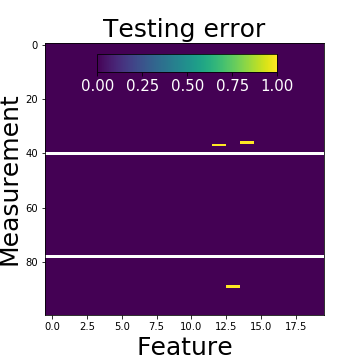
\includegraphics[width=0.24\textwidth]{{images/new_8-31-2020/short_test_S_title_SPCA_prediction_with_RPCA_first_selected_m_200_n_20_k_6_noiseSize_0.000000_numAnoms_10_sizeAnoms_1.000000_right}.png}
\caption{An SPCA prediction with RPCA first.  
%Note that, similar to PCA with RPCA, both only rows are incorrect because of anomalies in the testing data.
Similar to Figure \ref{fig:error_SPCA_prediction_without_RPCA_first_selected} the top left shows the anomalies in the training data, and the top right shows the anomalies in the testing data.  However, because of our use of RPCA \emph{we are able to choose columns with no anomalies} to train our SPCA algorithm.  Accordingly, in the bottom two figures errors only appear when there are anomalies in the testing data and the rest of the testing data is perfectly recovered.}
\label{fig:error_SPCA_prediction_with_RPCA_first_selected}
\end{figure}

%%%%%%%%%%%%%%%%%%%%%%%%%%%%%%%%%%%%%%%%%%%%%%%%%%%%%%%%%%%%%%%%

% \begin{figure}
%     \centering
%     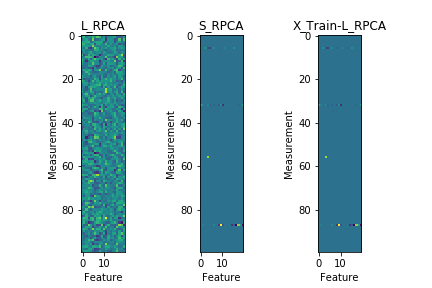
\includegraphics[width=0.45\textwidth]{{images/new_7-26-2020/short_train_S_m_200_n_20_k_10_noiseSize_0.000000_numAnoms_10_sizeAnoms_1.000000}.png}
%     \caption{Caption}
%     \label{fig:my_label}
% \end{figure}

%%%%%%%%%%%%%%%%%%%%%%%%%%%%%%%%%%%%%%%%%%%%%%%%%%%%%%%%%%%%%%%%

Figures \ref{fig:real_data} shows the results of our methodologies running on real healthcare provided data.  In the left of Figure \ref{fig:real_data} we see that the (approximate) rank of the real-world data is $10$.   Accordingly, one could imagine reaping the benefits of having access to all $34$ health-care metrics by just measuring $10$ healthcare metrics, with the commensurate saving the burden of data gathering.  In addition, as we do not know where the true anomalies, if any occur, we test our methodology by adding anomalies of our own.  We then tune $\lambda$ to the largest value for which these anomalies are detected in $S$.\footnote{Note, the real-world data we analyze here is noisier and smaller then RPCA is classically applied to.  However, note we observe that RPCA does provide useful insights into the data even in this domain even though we use different $\lambda$ values for rank and anomaly detection.} As one may observe, our method detects our added anomalies perfectly and, as such, makes the other detected anomalies, by way of their presence in the $S$ matrix, highly suspect and worthy of further investigation.   

In the right of Figure \ref {fig:real_data}
%{fig:real_data_rank} 
we show anomalies in the real data.  Specifically, the columns of the right side of Figure \ref {fig:real_data} can be translated to indicate that the following features had anomalies: 

\begin{itemize}
\item 
%Column 16 corresponds to ACO40. This feature is in the GPRO (web reported measure) category and is specifically a measure for 
“Depression Remission at 12 months”

\item 
%Column 4 corresponds to ACO17. This feature is in the GPRO (web reported measure) category and is specifically a measure for 
GPRO: “Preventive Care and Screening”: Tobacco Use: Screening and Cessation Information”  %\footnote{This feature was actually anomalous \emph{twice} even in such a small data set and %hence is especially problematic.} -- Not true.  This was a Melanie transciption errror cf 29 Jul 2020 3:46 pm

\item 
%Column 24 corresponds to ACO7. This feature is in the CAHPS survey category a 
CAHPS: "Health Status/Functional status"
%“Preventive Care and Screening”: Tobacco Use: Screening and Cessation Information”
%\todo [color = yellow]{Melanie needs to fix this: measures don't match listing earlier in %paper and columns are inconsistent DONE}
\item 
%Column 18 corresponds to  ACO1. This feature is in the CAHPS survey category and is specifically a measure for 
“CAHPS: Getting Timely Care, Appointments and Information”

\item 
%Column 31 corresponds to ACO36. . This feature is in the EHR (in this case, a calculation made from claims data) category and is specifically a measure for 
EHR: “All-Cause Unplanned Admissions for Patients with Diabetes”
\end{itemize}

Based on the data, these features should be avoided as required metrics.

% Clearly based upon these results, it would be important to not measure....
%\todo [ color = red]{LS:  Finish this up.  You can mention that the other columns are cleaner and perhaps better choices for measurement.  However, AC017 has multiple anomalies, and is therefore %not a good choice. DONE}

%\todo [ color = red]{RP, LS: MITRE ask: You assume or conclude that they are true anomalies, but you don't actually know that DONE}

\begin{figure}
\begin{subfigure}{.5\textwidth}
    \centering
    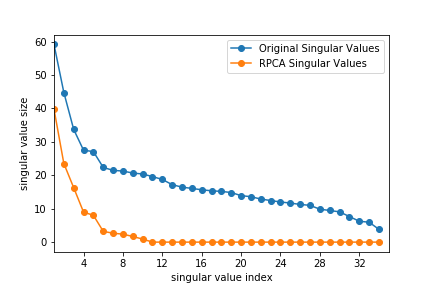
\includegraphics[width=0.8\textwidth]{images/new_7-26-2020/real_data_svd.png}
    \label{fig:real_data_rank}
\end{subfigure}
\begin{subfigure}{.5\textwidth}
    \centering
    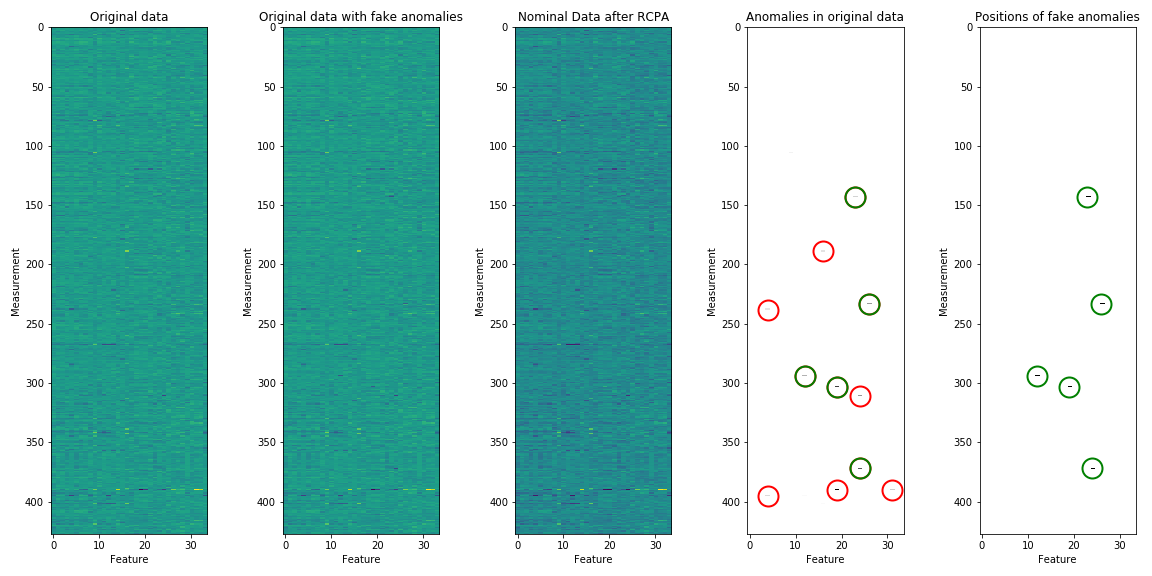
\includegraphics[width=1.0\textwidth]{images/new_7-26-2020/real_data.png}
    \label{fig:real_data_anomalie}
\end{subfigure}
    \caption{An example of RPCA analysis on real data.  The blue curve corresponds to the singular values computed if PCA only were applied to the data.  The orange curve corresponds to the singular values computed after the RPCA processing.  This example uses a small $\lambda=0.9/\sqrt{max(m,n)}$ to emphasize the low-rank structure. 
    %An example of RPCA analysis on real data.   
    We add anomalies of our own and choose the smallest $\lambda$ that recovers our added anomalies.  The entries in red circles are anomalies in the actual data. This example uses a large $\lambda=6.0/\sqrt{max(m,n)}$ to emphasize anomalies. }
    \label{fig:real_data}
\end{figure}
%\todo [color = red, inline] {Please check the caption of Fig 8: Two different lambda formulae are given.  Is that correct?}
%\todo[color=yellow,inline]{LS:  What do we learn from fig 16 in terms of recommended policy?
%We should summarize that we can recover placed anomalies in the real data in the intro. Also, summarize recommendation.}
%\todo[inline]{RCP:  I think we need another graphic to support the claim that we believe using our analysis that we only need X metrics and that the impact of that will be Y.  For example a singular value plot for the real data.  However, I am not sure this is very clear.}


% \begin{figure}[H]
%     \centering
%     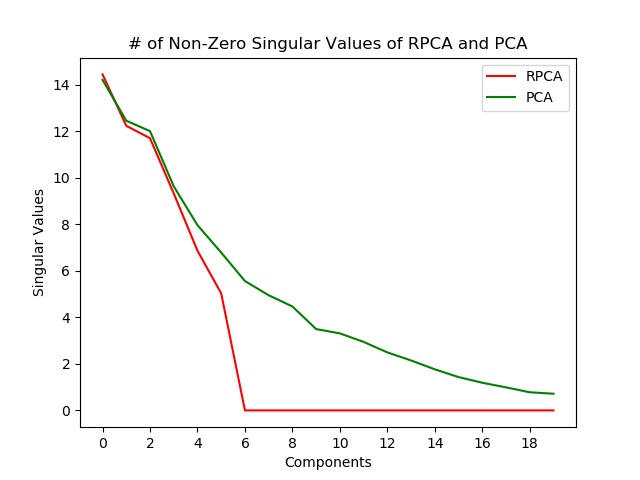
\includegraphics[width=50mm, scale=0.5]{Singular_Value_Plot_Test_120AnomSize5.jpg}
%     \caption{Singular Value comparison for PCA and RPCA on synthetic data with 3 percent anomalies of size 5}
%     \label{fig:singvaltrain1205}
% \end{figure}

% \begin{figure}[H]
%     \centering
%     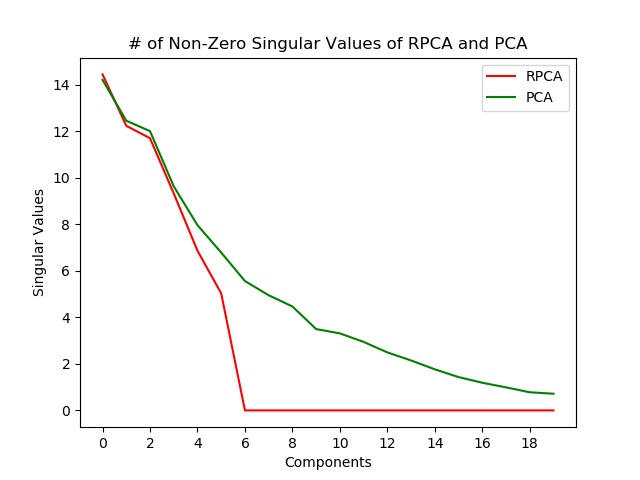
\includegraphics[width=50mm, scale=0.5]{Singular_Value_Plot_Test_120AnomSize5.jpg}
%     \caption{Singular Value comparison for PCA and RPCA on synthetic data with 3 percent anomalies of size 5}
%     \label{fig:singvaltrain1205}
% \end{figure}

% \begin{figure}[H]
% \begin{minipage}[b]{0.45\linewidth}
%     \centering
%     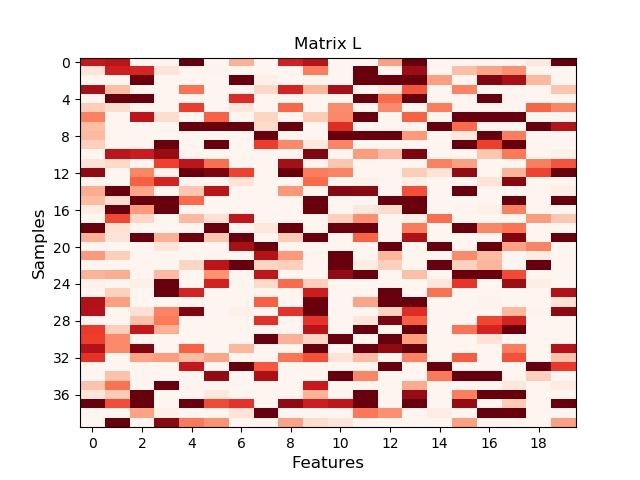
\includegraphics[width=45mm, scale=0.5]{L_120AnomSize5.jpg}
%     \caption{Low-Rank Matrix resulting from RPCA on synthetic data with 3 percent anomalies of size 5}
%     \label{fig:Ltrain1205}
% \end{minipage}
% \quad
% \begin{minipage}[b]{0.45\linewidth}
%     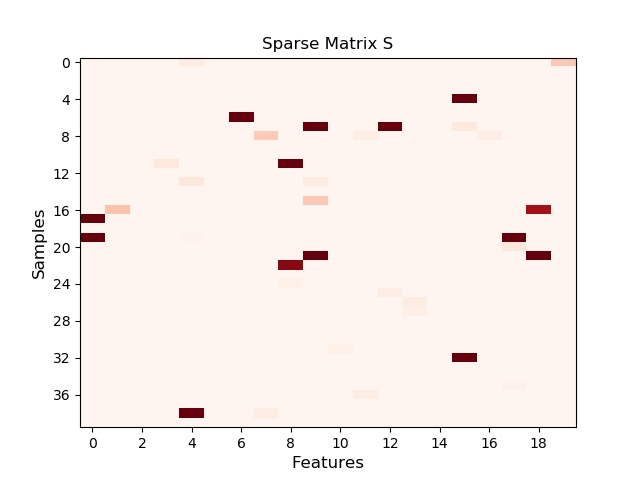
\includegraphics[width=45mm, scale=0.5]{S_120AnomSize5.jpg}
%     \caption{Sparse Matrix resulting from RPCA on synthetic data with 3 percent anomalies of size 5}
%     \label{fig:Strain1205}
% \end{minipage}
% \end{figure}

% \begin{figure}[H]
% \begin{minipage}[b]{0.45\linewidth}
%     \centering

%     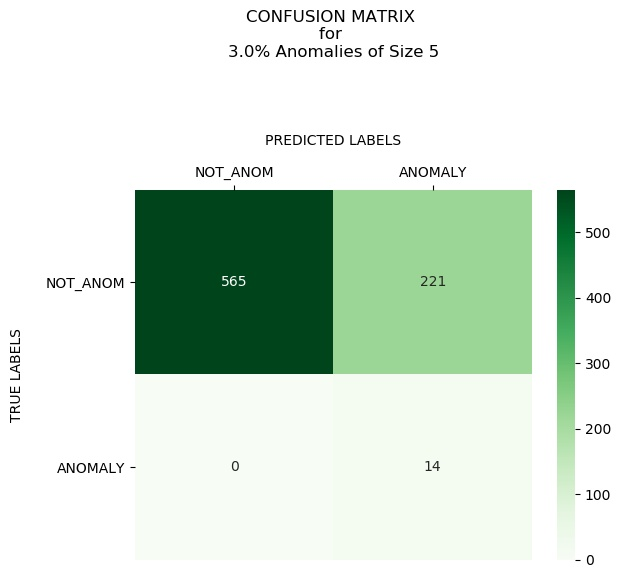
\includegraphics[width=50mm, scale=0.5]{cmPCATest_120AnomSize5.jpg}
%     \caption{Confusion Matrix resulting from PCA on synthetic data with 3 percent anomalies of size 5}
%     \label{fig::CMtrainPCA1205}
% \end{minipage}
% \quad
% \begin{minipage}[b]{0.45\linewidth}
%     \centering
%     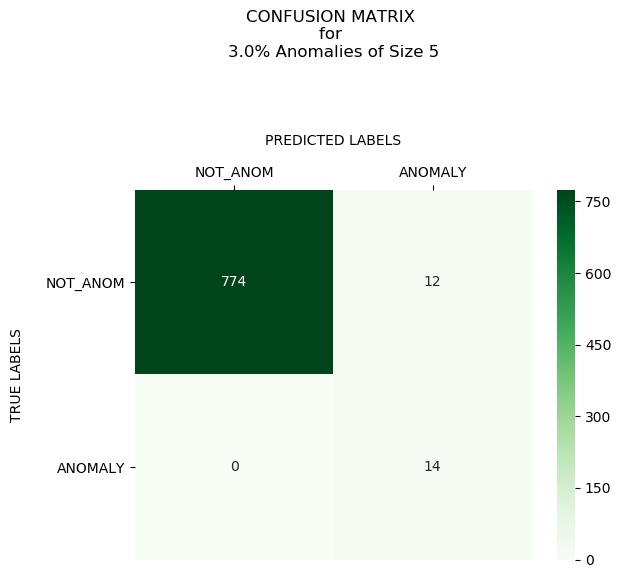
\includegraphics[width=50mm, scale=0.5]{cmRPCATest_120AnomSize5.jpg}
%     \caption{Confusion Matrix resulting from RPCA on synthetic data with 3 percent anomalies of size 5}
%     \label{fig::CMtrainRPCA125}
% \end{minipage}
% \end{figure}

% % Insert Figures for three percent anomalies size 10

% \begin{figure}[H]
%     \centering
%     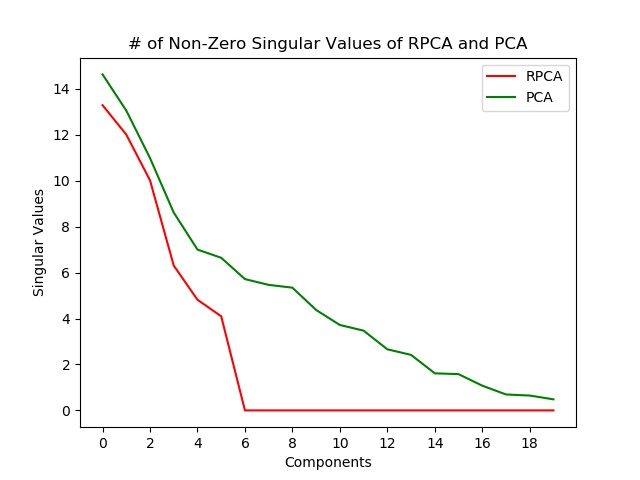
\includegraphics[width=50mm, scale=0.5]{Singular_Value_Plot_Test_120AnomSize10.jpg}
%     \caption{Singular Value comparison for PCA and RPCA on synthetic data with 3 percent anomalies of size 10}
%     \label{fig:singvaltrain12010}
% \end{figure}
% \begin{figure}[H]
% \begin{minipage}[b]{0.45\linewidth}
%     \centering
%     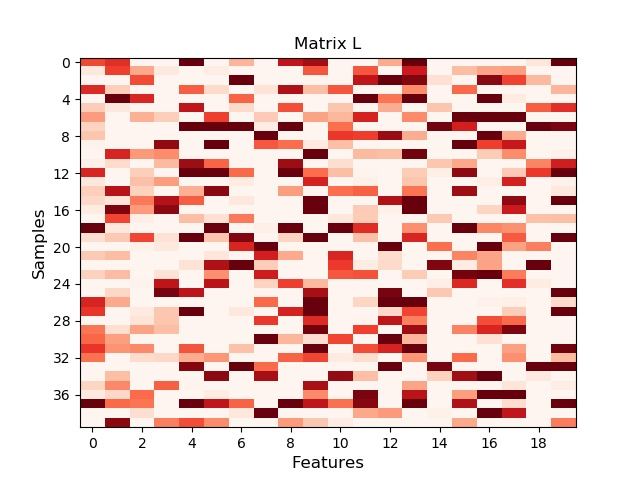
\includegraphics[width=45mm, scale=0.5]{L_120AnomSize10.jpg}
%     \caption{Low-Rank Matrix resulting from RPCA on synthetic data with 3 percent anomalies of size 10}
%     \label{fig:Ltrain12010}
% \end{minipage}
% \quad
% \begin{minipage}[b]{0.45\linewidth}
%     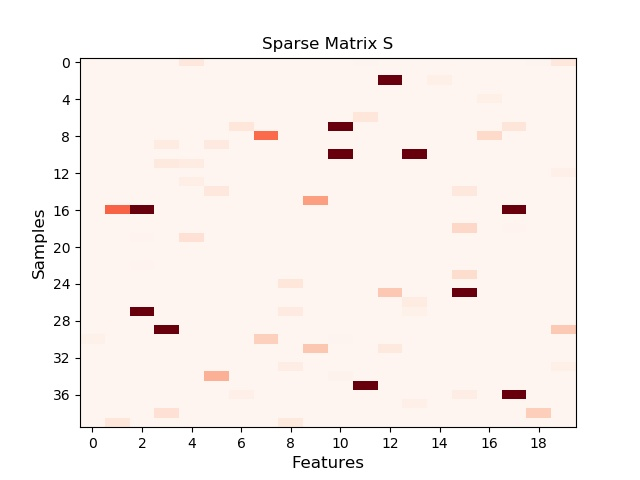
\includegraphics[width=45mm, scale=0.5]{S_120AnomSize10.jpg}
%     \caption{Sparse Matrix resulting from RPCA on synthetic data with 3 percent anomalies of size 10}
%     \label{fig:Strain12010}
% \end{minipage}
% \end{figure}

% \begin{figure}[H]
% \begin{minipage}[b]{0.45\linewidth}
%     \centering

%     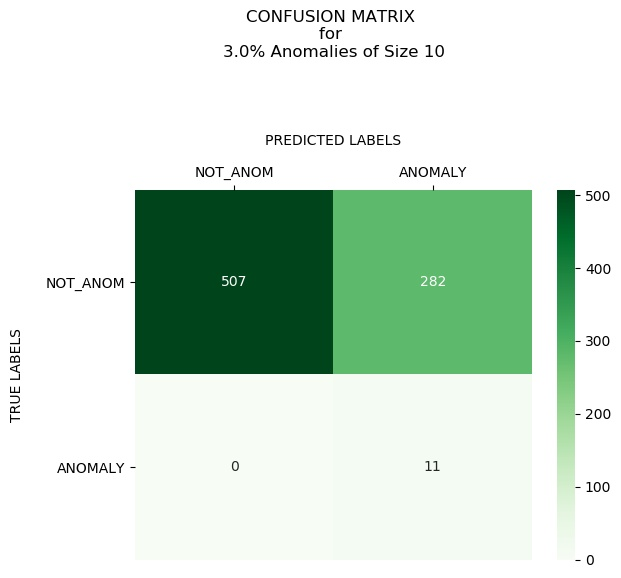
\includegraphics[width=50mm, scale=0.5]{cmPCATest_120AnomSize10.jpg}
%     \caption{Confusion Matrix resulting from PCA on synthetic data with 3 percent anomalies of size 10}
%     \label{fig::CMtrainPCA12010}
% \end{minipage}
% \quad
% \begin{minipage}[b]{0.45\linewidth}
%     \centering
%     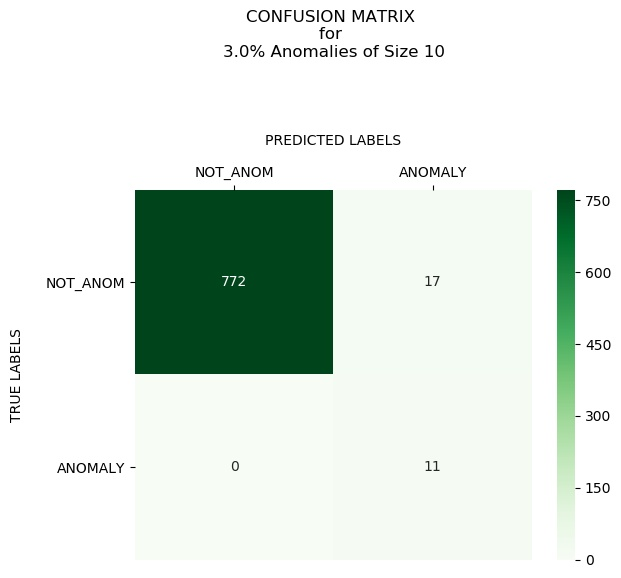
\includegraphics[width=50mm, scale=0.5]{cmRPCATest_120AnomSize10.jpg}
%     \caption{Confusion Matrix resulting from RPCA on synthetic data with 3 percent anomalies of size 10}
%     \label{fig::CMtrainRPCA12010}
% \end{minipage}
% \end{figure}

% % Insert Figures for ten percent anomalies size 5

% \begin{figure}[H]
%     \centering
%     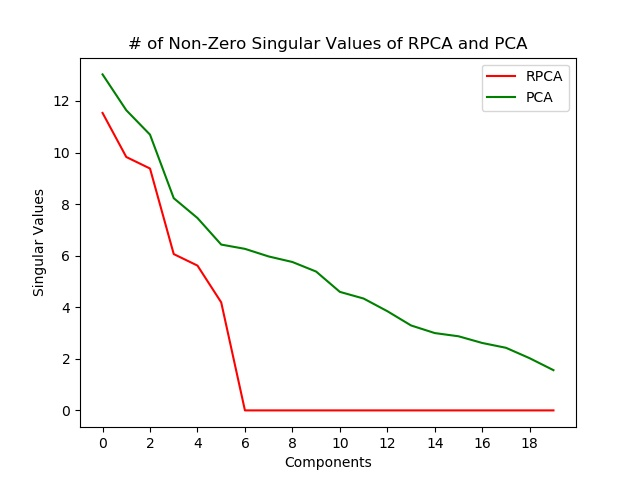
\includegraphics[width=50mm, scale=0.5]{Singular_Value_Plot_Test_400AnomSize5.jpg}
%     \caption{Singular Value comparison for PCA and RPCA on synthetic data with 10 percent anomalies of size 5}
%     \label{fig:singvaltrain4005}
% \end{figure}
% \begin{figure}[H]
% \begin{minipage}[b]{0.45\linewidth}
%     \centering
%     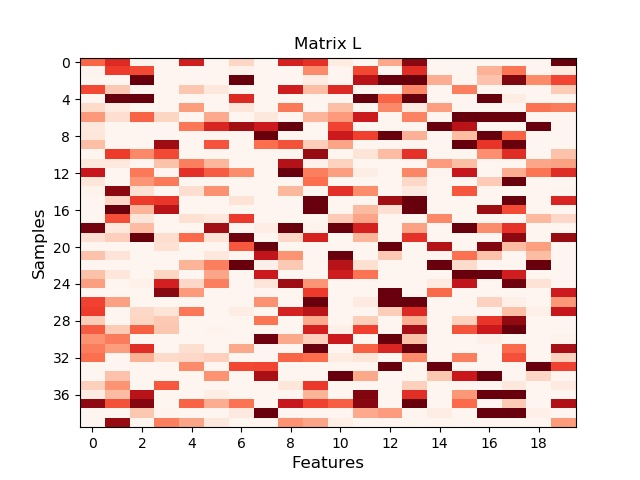
\includegraphics[width=45mm, scale=0.5]{L_400AnomSize5.jpg}
%     \caption{Low-Rank Matrix resulting from RPCA on synthetic data with 10 percent anomalies of size 5}
%     \label{fig:Ltrain4005}
% \end{minipage}
% \quad
% \begin{minipage}[b]{0.45\linewidth}
%     \includegraphics[width=45mm, scale=0.5]{S_400AnomSize5.jpg}
%     \caption{Sparse Matrix resulting from RPCA on synthetic data with 10 percent anomalies of size 5}
%     \label{fig:Strain4005}
% \end{minipage}
% \end{figure}

% \begin{figure}[H]
% \begin{minipage}[b]{0.45\linewidth}
%     \centering

%     \includegraphics[width=50mm, scale=0.5]{cmPCATest_400AnomSize5.jpg}
%     \caption{Confusion Matrix resulting from PCA on synthetic data with 10 percent anomalies of size 5}
%     \label{fig::CMtrainPCA4005}
% \end{minipage}
% \quad
% \begin{minipage}[b]{0.45\linewidth}
%     \centering
%     \includegraphics[width=50mm, scale=0.5]{cmRPCATest_400AnomSize5.jpg}
%     \caption{Confusion Matrix resulting from RPCA on synthetic data with 10 percent anomalies of size 5}
%     \label{fig::CMtrainRPCA4005}
% \end{minipage}
% \end{figure}

% % Insert Figures for ten percent anomalies size 10

% \begin{figure}[H]
%     \centering
%     \includegraphics[width=50mm, scale=0.5]{Singular_Value_Plot_Test_400AnomSize10.jpg}
%     \caption{Singular Value comparison for PCA and RPCA on synthetic data with 10 percent anomalies of size 10}
%     \label{fig:singvaltrain40010}
% \end{figure}
% \begin{figure}[H]
% \begin{minipage}[b]{0.45\linewidth}
%     \centering
%     \includegraphics[width=45mm, scale=0.5]{L_400AnomSize10.jpg}
%     \caption{Low-Rank Matrix resulting from RPCA on synthetic data with 10 percent anomalies of size 10}
%     \label{fig:Ltrain40010}
% \end{minipage}
% \quad
% \begin{minipage}[b]{0.45\linewidth}
%     \includegraphics[width=45mm, scale=0.5]{S_400AnomSize10.jpg}
%     \caption{Sparse Matrix resulting from RPCA on synthetic data with 10 percent anomalies of size 10}
%     \label{fig:Strain40010}
% \end{minipage}
% \end{figure}

% \begin{figure}[H]
% \begin{minipage}[b]{0.45\linewidth}
%     \centering

%     \includegraphics[width=50mm, scale=0.5]{cmPCATest_400AnomSize10.jpg}
%     \caption{Confusion Matrix resulting from PCA on synthetic data with 10 percent anomalies of size 10}
%     \label{fig::CMtrainPCA40010}
% \end{minipage}
% \quad
% \begin{minipage}[b]{0.45\linewidth}
%     \centering
%     \includegraphics[width=50mm, scale=0.5]{cmRPCATest_400AnomSize10.jpg}
%     \caption{Confusion Matrix resulting from RPCA on synthetic data with 10 percent anomalies of size 10}
%     \label{fig::CMtrainRPCA40010}
% \end{minipage}
% \end{figure}

% \todo[inline]{Add MSE plots of outliers against error plot data csv files}
% \todo[inline]{Add results for Deon's combinatorial approach}
% \todo[inline]{RCP: Add approach for real data}
% \todo[inline]{Do Paffenroth insertions: add anomalies and show that we found them}
% \todo[inline]{Add results for real data: What does PCA/RPCA/Gurobi find}

\section{Conclusions}

This work presents a new research path to explore how modern optimization methods can help complement medical and policy judgment when seeking to reduce health metric burdens.  Our methodology recommends  the minimum selection of health metrics from a proposed set of candidates when there is reason to expect confounding measurement errors in the data.

In particular, empirical examples on synthetic data show our approach was the only method tested herein that found all possible anomalies with no false alarms and perfectly computed the required reduced number of metrics needed without appreciable loss of information.   In particular, we developed empirical evidence that using new modern optimization methods such as RPCA can be effective at complementing classic techniques such as PCA and SPCA in achieve multiple goals simultaneously when the individual techniques cannot provide all of the functionality that is required.

%\todo [ color = orange,inline]{RCP: MITRE ask: so how many metrics were you able to identify as redundant.  That seems to be the entire oint of the paer, but it isn't addressed directly DONE but maybe we should revist}

%\todo[color=yellow,inline]{LS: Conclusions: I think we should be more assertive:  }

\section{Acknowledgment}
% ANONYMOUS
The authors wish to thank Dr. Allen Leavens, (MITRE) for introducing us to the challenges of health reporting burdens as well as the introducing us to the Center for Medicare and Medicaid Services (CMS)'s public use dataset related to the Shared Saving Program Accountable Care Organization (ACO).   They also thank Brady Collea for his discussion and  assistance with the many experiments performed related to this work.

% Approved for Public Release. Distribution Unlimited. Case Number 20-1958.$\copyright$ 2020 The MITRE Corporation. All Rights Reserved.

\bibliographystyle{IEEEtran}
\bibliography{ICMLA}

%\newpage
%\listoftodos[Notes]
\end{document}
